\documentclass[11pt,a4paper]{article}

% ============================================================================
% PAQUETES
% ============================================================================
\usepackage[utf8]{inputenc}
\usepackage[spanish]{babel}
\usepackage[T1]{fontenc}
\usepackage{amsmath,amsfonts,amssymb}
\usepackage{graphicx}
\usepackage{booktabs}
\usepackage{float}
\usepackage{hyperref}
\usepackage{geometry}
\usepackage{setspace}
\usepackage{natbib}
\usepackage{caption}
\usepackage{subcaption}
\usepackage{multirow}
\usepackage{array}
\usepackage[dvipsnames]{xcolor}
\usepackage{fancyhdr}
\usepackage{longtable}
\usepackage{pdflscape}
\usepackage{titlesec}
\usepackage{enumitem}
\usepackage{tcolorbox}
\usepackage{pifont}
\newcommand{\cmark}{\ding{51}}
\newcommand{\xmark}{\ding{55}}
% Comando para términos del glosario con hipervínculo
\newcommand{\gterm}[2]{\hyperref[glos:#1]{#2}}


% Configuracion de pagina
\geometry{margin=2.5cm, headheight=14pt}
\setstretch{1.5}

% Configuracion de encabezados
\pagestyle{fancy}
\fancyhf{}
\fancyhead[L]{\small\textit{Aprendizaje Automático para Generación de Alfa en el S\&P 500}}
\fancyhead[R]{\small\thepage}
\renewcommand{\headrulewidth}{0.4pt}

% Configuracion de hyperref
\hypersetup{
    colorlinks=true,
    linkcolor=blue!70!black,
    filecolor=magenta,
    urlcolor=cyan!70!black,
    citecolor=blue!70!black
}

% Formato de secciones
\titleformat{\section}{\large\bfseries}{\thesection.}{0.5em}{}
\titleformat{\subsection}{\normalsize\bfseries}{\thesubsection}{0.5em}{}
\titleformat{\subsubsection}{\normalsize\itshape}{\thesubsubsection}{0.5em}{}

% ============================================================================
% DOCUMENTO
% ============================================================================
\begin{document}

% ============================================================================
% TITULO
% ============================================================================
\thispagestyle{empty}
\begin{center}

\vspace*{0.8cm}

{\LARGE\bfseries Desafiando la Eficiencia del Mercado:\par}
\vspace{0.5cm}
{\Large\bfseries Aprendizaje Automático para Predicción Direccional\\ y Generación de Alfa en el S\&P 500\par}

\vspace{1.2cm}

{\large David González Canón\par}
\vspace{0.4cm}
{\normalsize Maestría en Inteligencia de Negocios para Finanzas\par}
\vspace{0.2cm}
{\normalsize Diciembre 2025\par}

\vspace{1.2cm}

\noindent\rule{0.9\textwidth}{0.5pt}

\vspace{0.8cm}

\end{center}

\begin{minipage}{0.95\textwidth}
\small
\setstretch{1.25}
\textbf{Resumen}

\vspace{0.3cm}

Este estudio investiga empíricamente la Hipótesis de Eficiencia de Mercado mediante un enfoque estructurado en dos hitos fundamentales. El \textbf{primer hito} consiste en entrenar 23 modelos de aprendizaje automático y profundo (incluyendo Ridge, XGBoost, LightGBM, \gterm{lstm}{LSTM}, TCN, y Transformers) para generar predicciones sobre los retornos del S\&P 500. El objetivo no es predecir con exactitud el valor del retorno de mañana, sino obtener suficiente precisión direccional para tomar decisiones de inversión. El \textbf{segundo hito} traduce estas predicciones en una estrategia de trading LONG-ONLY que aprovecha el apalancamiento disponible en ETFs para generar alfa positivo después de costos de transacción.

El proceso de ingeniería de características transforma 92 variables macroeconómicas, financieras y de sentimiento de Bloomberg Terminal en 647 predictores. Esta transformación incluye técnicas diversas como indicadores técnicos clásicos y estimadores de volatilidad basados en precios OHLC (Parkinson, Garman-Klass, Rogers-Satchell, Yang-Zhang).

Cuatro de veintitrés modelos superan al benchmark pasivo, demostrando que la dificultad de superar al mercado es real pero no insuperable. Los hallazgos presentan evidencia empírica de que técnicas de aprendizaje automático pueden capturar patrones direccionales explotables en retornos de mercado, contribuyendo al debate sobre la validez de la Hipótesis de Eficiencia de Mercado.

\end{minipage}

\vspace{0.8cm}

\begin{center}
\noindent\rule{0.9\textwidth}{0.5pt}
\end{center}

\newpage

\vspace*{0.5cm}

\textbf{Palabras clave:} Hipótesis de Eficiencia de Mercado, Aprendizaje Automático, Aprendizaje Profundo, Pronóstico de Series Temporales, Análisis Técnico, Generación de Alfa, S\&P 500, Finanzas Cuantitativas, ETFs Apalancados, Gestión de Riesgo

\vspace{0.5cm}

\textbf{Clasificación JEL:} G14, G17, C45, C53

\vspace{1cm}

% ============================================================================
% TABLA DE CONTENIDOS
% ============================================================================
\tableofcontents
\newpage

% ============================================================================
% 1. INTRODUCCION
% ============================================================================
\section{Introducción}

\subsection{Contexto y Motivación}

La Hipótesis de Eficiencia de Mercado (HEM), formalizada por \citet{fama1970} hace más de cinco décadas, permanece como una de las proposiciones más influyentes y debatidas en la economía financiera contemporánea. En su formulación más estricta, la hipótesis postula que los precios de los activos incorporan instantánea y completamente toda la información disponible, haciendo imposible la obtención de rendimientos anormales sistemáticos a través de cualquier estrategia de trading basada en datos históricos o información pública.

Sin embargo, el panorama empírico ha evolucionado considerablemente desde el trabajo seminal de Fama. La proliferación de anomalías documentadas, la sofisticación creciente de las técnicas de aprendizaje automático, y la disponibilidad de conjuntos de datos cada vez más ricos han reavivado el debate fundamental: ¿procesan realmente los mercados financieros la información de manera eficiente, o existen ineficiencias persistentes susceptibles de explotación por inversores sofisticados?

Este estudio contribuye a este debate mediante un enfoque empírico estructurado en \textbf{dos hitos fundamentales}:

\textbf{Hito 1 -- Predicción:} Entrenar múltiples modelos de aprendizaje automático y profundo (23 en total) para generar predicciones sobre los retornos del S\&P 500. El objetivo no es predecir con exactitud el valor numérico del retorno de mañana, sino obtener suficiente \textit{precisión direccional} para tomar decisiones de inversión.

\textbf{Hito 2 -- Implementación:} Traducir las predicciones de los modelos en una estrategia de trading práctica que aproveche el apalancamiento disponible en ETFs para generar alfa positivo después de costos de transacción realistas.

Este enfoque reconoce una distinción crucial: mientras que predecir el retorno exacto del mercado puede ser imposible, identificar la \textit{dirección} con precisión suficiente puede ser económicamente explotable cuando se combina con una estrategia de posicionamiento inteligente.

\subsection{La Relevancia del Debate sobre Eficiencia de Mercado}

El debate sobre la eficiencia de mercado trasciende el ámbito puramente académico y tiene implicaciones profundas para la industria de gestión de activos, la regulación financiera y las decisiones de inversión individuales. Si los mercados son verdaderamente eficientes, los gestores activos de fondos destruyen valor para sus clientes a través de comisiones y costos de transacción sin generar rendimientos superiores al mercado. En este escenario, la inversión pasiva a través de fondos indexados representaría la estrategia óptima para todos los inversores.

Por el contrario, si existen ineficiencias sistemáticas y explotables, surge la posibilidad de que estrategias cuantitativas sofisticadas puedan generar rendimientos ajustados por riesgo superiores. Esta posibilidad ha impulsado el crecimiento exponencial de la industria de hedge funds cuantitativos, que según estimaciones de la industria gestiona más de un billón de dólares en activos globalmente \citep{preqin2024}.

La presente investigación se sitúa en la intersección de estos debates al examinar si las técnicas más avanzadas de aprendizaje automático, combinadas con indicadores técnicos probados en la práctica, pueden identificar patrones predecibles en los retornos del mercado de valores, patrones que al ser utilizados con una estrategia bien definida pueden generar retornos por encima del mercado.

\subsection{Contribuciones al Conocimiento}

Este estudio realiza múltiples contribuciones originales al cuerpo de conocimiento existente en la intersección de aprendizaje automático y finanzas cuantitativas.

\paragraph*{Marco metodológico de dos hitos.} La literatura existente frecuentemente confunde la capacidad predictiva de un modelo con su rentabilidad práctica. Este estudio introduce una separación explícita entre la fase de predicción (entrenamiento y evaluación de modelos) y la fase de implementación (traducción de predicciones a posiciones de trading). Esta distinción es fundamental porque un modelo con excelentes métricas predictivas puede fracasar en la práctica debido a costos de transacción, timing inadecuado, o dimensionamiento incorrecto de posiciones. Al evaluar cada fase de manera independiente, se identifican con precisión las fuentes de alfa y los puntos de falla potenciales.

\paragraph*{Comparación exhaustiva de arquitecturas.} Mientras que estudios previos típicamente comparan un número limitado de modelos dentro de una misma familia metodológica, este trabajo evalúa 23 modelos que abarcan el espectro completo de técnicas disponibles: desde regresión lineal regularizada hasta arquitecturas de deep learning de última generación (Transformers, TCN, LSTM bidireccionales). Esta amplitud permite identificar patrones sistemáticos sobre qué familias de modelos funcionan mejor en el contexto específico de predicción de retornos del S\&P 500, proporcionando orientación práctica para investigadores y practicantes.

\paragraph*{Ingeniería de características multi-técnica.} A diferencia de enfoques que dependen de una única metodología de extracción de características, este estudio implementa un pipeline que integra múltiples técnicas complementarias: indicadores técnicos clásicos, estimadores de volatilidad basados en precios OHLC (Parkinson, Garman-Klass, Rogers-Satchell, Yang-Zhang), el sistema \gterm{triple-screen}{Triple Screen} de Elder, y correlaciones cross-asset dinámicas. Esta diversidad metodológica maximiza la información predictiva extraída de los datos disponibles y permite que los modelos capturen diferentes aspectos de la dinámica de mercado.

\paragraph*{Análisis de costos de implementación.} Un aspecto frecuentemente ignorado en la literatura académica es el impacto de los costos de transacción en la viabilidad práctica de las estrategias. Este estudio incorpora un modelo de costos conservador que incluye spreads bid-ask, comisiones, y slippage, demostrando que el alfa teórico puede erosionarse significativamente---o incluso desaparecer---cuando se consideran fricciones realistas. Esta contribución es crucial para distinguir entre resultados académicamente interesantes y estrategias genuinamente implementables.

\paragraph*{Evidencia sobre simplicidad versus complejidad.} Contrariamente a la intuición de que modelos más sofisticados deberían producir mejores predicciones, los resultados demuestran que un modelo simple (Ridge) supera consistentemente a arquitecturas complejas de deep learning. Este hallazgo se alinea con evidencia reciente en la literatura \citep{zeng2023} y tiene implicaciones prácticas importantes: en entornos con bajo ratio señal-ruido como los mercados financieros, la regularización implícita de modelos simples puede ser más valiosa que la flexibilidad de arquitecturas complejas.

\paragraph*{La Paradoja del Directional Accuracy.} Uno de los hallazgos más contraintuitivos de este estudio desafía una suposición común en la literatura: que un modelo que predice correctamente la dirección del mercado con mayor frecuencia debería generar mayores retornos. Los resultados empíricos revelan lo contrario---la correlación entre \gterm{da}{Directional Accuracy (DA)} y rentabilidad es negativa ($\rho = -0.14$). Modelos con DA superior al 54\% generaron retornos negativos, mientras que modelos con DA cercano al 51\% lograron los mejores retornos. La explicación radica en que el DA trata todos los días como iguales, ignorando la magnitud de los movimientos y el tamaño de las posiciones. Un modelo puede acertar frecuentemente en días de movimientos pequeños pero fallar en los días críticos de alta volatilidad. Se propone \gterm{da3x}{DA3x}---el hit rate calculado únicamente cuando el modelo toma posiciones apalancadas---como métrica alternativa que captura la calidad de las predicciones en los momentos que realmente determinan la rentabilidad.

\subsection{Estructura del Documento}

El documento está organizado siguiendo la lógica de los dos hitos fundamentales:

\textbf{Contexto teórico:} La Sección 2 presenta una revisión de la literatura relevante sobre eficiencia de mercado, anomalías documentadas, y aplicaciones de aprendizaje automático en finanzas.

\textbf{Hito 1 -- Predicción:} La Sección 3 describe la metodología de predicción: fuentes de datos, ingeniería de características (incluyendo las diversas técnicas empleadas para extraer información de los datos), especificaciones de los 23 modelos, y el marco de evaluación.

\textbf{Hito 2 -- Implementación:} La Sección 4 presenta la estrategia de posiciones discretas y los resultados empíricos. La Sección 5 analiza detalladamente los costos de transacción y su impacto en la rentabilidad real.

\textbf{Discusión y cierre:} La Sección 6 discute las implicaciones para el debate sobre eficiencia de mercado. La Sección 7 examina limitaciones y robustez. La Sección 8 concluye con un resumen de hallazgos. Los apéndices proporcionan documentación técnica detallada.

% ============================================================================
% 2. REVISION DE LITERATURA Y FUNDAMENTOS TEORICOS
% ============================================================================
\section{Revisión de Literatura y Fundamentos Teóricos}

\subsection{La Hipótesis de Eficiencia de Mercado: Origen y Evolución}

\subsubsection{Fundamentos Conceptuales}

La noción de que los precios de mercado reflejan la información disponible tiene raíces que se remontan a los trabajos pioneros de Louis Bachelier a principios del siglo XX. Sin embargo, la formulación moderna de la Hipótesis de Eficiencia de Mercado se atribuye principalmente a Eugene Fama, cuyo artículo seminal de 1970 estableció el marco conceptual que domina el pensamiento financiero hasta el día de hoy.

\citet{fama1970} definió un mercado eficiente como aquel en el que los precios ``reflejan completamente'' la información disponible. Esta definición aparentemente simple encierra profundas implicaciones para la práctica de inversión y la teoría financiera. Fama distinguió tres formas de eficiencia de mercado, cada una correspondiente a un conjunto diferente de información:

La \textbf{eficiencia en forma débil} postula que los precios actuales incorporan completamente toda la información contenida en la secuencia histórica de precios. Bajo esta forma de eficiencia, el análisis técnico---la práctica de usar patrones de precios históricos para predecir movimientos futuros---debería ser incapaz de generar rendimientos anormales sistemáticos. Los precios seguirían un proceso de caminata aleatoria, haciendo que cualquier patrón aparente sea el resultado de coincidencia estadística más que de una relación causal explotable.

La \textbf{eficiencia en forma semi-fuerte} extiende esta noción al postular que los precios reflejan toda la información públicamente disponible, incluyendo estados financieros, anuncios corporativos, indicadores macroeconómicos, y cualquier otra información accesible sin privilegios especiales. Bajo esta forma de eficiencia, el análisis fundamental---el estudio de factores económicos, financieros y cualitativos para determinar el valor intrínseco de un activo---tampoco debería generar rendimientos anormales consistentes.

La \textbf{eficiencia en forma fuerte} representa la proposición más extrema: los precios reflejan toda la información, incluyendo información privada o ``insider''. Esta forma implica que ni siquiera los insiders corporativos podrían obtener beneficios sistemáticos de su acceso privilegiado a información no pública.

\subsubsection{El Problema del ``Joint Hypothesis''}

Un desafío fundamental en las pruebas empíricas de la HEM, reconocido por el propio Fama, es el llamado problema de la hipótesis conjunta. Cualquier prueba de eficiencia de mercado es simultáneamente una prueba del modelo de equilibrio utilizado para definir ``rendimientos normales''. Si observamos rendimientos que aparentan ser anormales, no podemos distinguir con certeza entre dos explicaciones: (1) el mercado es ineficiente, o (2) el modelo de equilibrio está mal especificado.

Este problema tiene implicaciones profundas para la interpretación de los resultados. Los rendimientos superiores que se documenta podrían representar verdadera ineficiencia de mercado (un fracaso en la incorporación eficiente de información), o podrían representar compensación por riesgo que los modelos no capturan adecuadamente. Volveremos a esta cuestión en la discusión de resultados.

\subsubsection{La Paradoja de Grossman-Stiglitz}

Una crítica teórica fundamental a la HEM fue planteada por \citet{grossman1980}, quienes demostraron la imposibilidad lógica de mercados perfectamente eficientes. Su argumento, conocido como la ``paradoja de la información'', procede de la siguiente manera:

Si los mercados fueran perfectamente eficientes y los precios reflejaran completamente toda la información disponible, entonces ningún inversor podría obtener rendimientos superiores mediante la adquisición y análisis de información. Pero si no existe beneficio en adquirir información---dado que los precios ya la reflejan---¿por qué los participantes del mercado pagarían por acceso a noticias financieras, servicios de análisis, terminales Bloomberg, o informes de corredores?

La paradoja revela una contradicción interna: si nadie tiene incentivos para recopilar información (porque no pueden beneficiarse de ella), entonces los precios no pueden reflejar esa información. Pero si los precios no reflejan la información, entonces sí existen oportunidades de beneficio, lo que motivaría la adquisición de información. \citet{grossman1980} concluyen que los mercados deben ser ``eficientemente ineficientes''---lo suficientemente ineficientes para compensar a quienes invierten en la adquisición de información, pero no tan ineficientes como para permitir ganancias excesivas después de considerar los costos de información.

Esta perspectiva tiene implicaciones directas para el presente estudio: la existencia de alfa positivo después de costos no contradice necesariamente una noción razonable de eficiencia de mercado, siempre que ese alfa represente compensación legítima por el esfuerzo de desarrollar y mantener sistemas predictivos sofisticados.

\subsection{Anomalías de Mercado y Evidencia Contra la HEM}

\subsubsection{El Catálogo de Anomalías}

A pesar del marco teórico elegante proporcionado por la HEM, décadas de investigación empírica han documentado numerosas ``anomalías''---patrones sistemáticos en los rendimientos que aparentemente contradicen las predicciones de eficiencia. \citet{dong2022} documentan más de 150 predictores de retornos que han sido identificados en la literatura académica, organizados en categorías que incluyen:

\textbf{Anomalías de momentum:} Jegadeesh y Titman (1993) documentaron que las acciones con rendimientos superiores en los 3-12 meses anteriores tienden a continuar superando a aquellas con rendimientos inferiores. Este efecto de momentum contradice directamente la forma débil de eficiencia, ya que implica que los rendimientos históricos contienen información predictiva sobre rendimientos futuros.

\textbf{Anomalías de valor:} Fama y French (1992) mostraron que las acciones con altas razones libro-a-mercado (``value stocks'') tienden a superar a aquellas con bajas razones (``growth stocks''). Esta anomalía de valor ha persistido a través de diferentes mercados y períodos de tiempo, aunque su magnitud ha disminuido desde su publicación original.

\textbf{Anomalías de tamaño:} Las acciones de empresas pequeñas han mostrado históricamente rendimientos superiores a las de empresas grandes, incluso después de ajustar por riesgo de mercado. Este ``efecto tamaño'' fue documentado originalmente por Banz (1981) y ha sido objeto de intenso escrutinio posterior.

\textbf{Anomalías de calendario:} Diversos efectos relacionados con el calendario han sido documentados, incluyendo el ``efecto enero'' (rendimientos anormalmente altos en enero), el ``efecto lunes'' (rendimientos negativos los lunes), y el ``efecto fin de mes'' (rendimientos positivos en los últimos días del mes).

\textbf{Anomalías de baja volatilidad:} Contrariamente a las predicciones del CAPM, las acciones de baja volatilidad han mostrado rendimientos ajustados por riesgo superiores a las de alta volatilidad. Este fenómeno, documentado por Ang et al. (2006), representa una de las contradicciones más directas a la teoría de valoración de activos estándar.

\subsubsection{Interpretaciones Alternativas de las Anomalías}

La existencia de anomalías no necesariamente implica ineficiencia de mercado. \citet{malkiel2003} argumenta que muchas anomalías aparentes pueden explicarse por:

\textbf{Compensación por riesgo:} Los rendimientos superiores podrían reflejar compensación por exposición a factores de riesgo que los modelos estándar no capturan. Bajo esta interpretación, las anomalías no representan ``dinero gratis'' sino primas de riesgo legítimas.

\textbf{Sesgo de publicación:} La literatura académica puede estar sesgada hacia la publicación de resultados que muestran predictibilidad, mientras que estudios que no encuentran patrones significativos permanecen en el ``cajón del escritorio''.

\textbf{Data mining:} Con suficientes variables y suficiente búsqueda, es estadísticamente inevitable encontrar patrones aparentemente significativos que son simplemente ruido estadístico. Este problema se exacerba por la práctica de probar múltiples hipótesis sin ajuste apropiado para comparaciones múltiples.

\textbf{Decaimiento de anomalías:} Muchas anomalías han mostrado debilitamiento o desaparición después de su publicación, consistente con la noción de que la publicación atrae capital que arbitra las ineficiencias.

\subsection{Aprendizaje Automático en Valoración de Activos}

\subsubsection{La Revolución del Machine Learning en Finanzas}

La aplicación del aprendizaje automático a la predicción financiera ha experimentado un crecimiento explosivo en la última década. \citet{gu2020} proporcionan un tratamiento comprehensivo de este campo, demostrando que las redes neuronales, el gradient boosting, y otros métodos no lineales superan sustancialmente a la regresión lineal en la predicción de rendimientos de acciones individuales. Su metodología, que emplea un gran número de características de empresas como predictores, se ha convertido en una referencia estándar en la literatura.

Un hallazgo clave de esta literatura concierne el trade-off entre complejidad del modelo y precisión predictiva en contextos financieros. Mientras que las arquitecturas de aprendizaje profundo han logrado éxitos notables en dominios como el reconocimiento de imágenes y el procesamiento del lenguaje natural, su aplicación a series temporales financieras ha producido resultados más mixtos.

\subsubsection{El Debate sobre Complejidad de Modelos}

\citet{zeng2023} presentan un hallazgo sorprendente que tiene implicaciones importantes para el presente estudio: un modelo simple de descomposición lineal (DLinear) que separa componentes de tendencia y estacionalidad antes de aplicar proyecciones lineales supera a arquitecturas sofisticadas basadas en Transformers en múltiples benchmarks de pronóstico de horizonte largo.

Este resultado tiene implicaciones importantes para las aplicaciones financieras. Las series temporales financieras son notoriamente ruidosas, con razones señal-a-ruido mucho más bajas que las encontradas en otras aplicaciones de aprendizaje automático. En tales entornos, la regularización implícita en arquitecturas de modelos más simples puede proporcionar ventajas sobre modelos complejos propensos a sobreajustar patrones espurios.

La lección que extraemos de esta literatura es que la sofisticación arquitectónica no garantiza mejor desempeño predictivo en finanzas. La selección de modelo debe estar guiada por validación empírica rigurosa más que por la novedad de la arquitectura.

\subsection{El Sistema Triple Screen de Alexander Elder}

\subsubsection{Origen y Filosofía}

Alexander Elder, psiquiatra de formación reconvertido en trader profesional, introdujo el sistema Triple Screen en su influyente libro ``Trading for a Living'' \citep{elder1993}. El sistema representa un enfoque sistemático para el timing de mercado que ha logrado amplia adopción entre traders profesionales durante más de tres décadas.

La filosofía subyacente del sistema se basa en la observación de que los mercados financieros exhiben tendencias y oscilaciones en múltiples marcos temporales simultáneamente. Un mercado puede estar en una tendencia alcista en el marco semanal mientras experimenta un retroceso temporal en el marco diario. Elder argumenta que los traders más exitosos son aquellos que pueden identificar estas dinámicas multi-temporales y posicionarse estratégicamente.

El nombre ``Triple Screen'' deriva del requisito de que una señal de trading debe pasar tres filtros secuenciales antes de la ejecución. Este enfoque de filtrado múltiple busca reducir las señales falsas que plagan los sistemas de trading basados en indicadores únicos.

\subsubsection{Primera Pantalla: Identificación de Tendencia}

La primera pantalla opera en un marco temporal superior al del trading (típicamente semanal para traders que operan en marco diario) y busca identificar la dirección de la tendencia dominante. Elder emplea principalmente dos indicadores para esta determinación:

\textbf{MACD (Moving Average Convergence Divergence):} Desarrollado por Gerald Appel, el MACD calcula la diferencia entre dos medias móviles exponenciales (típicamente de 12 y 26 períodos) y la compara con una línea de señal (media móvil exponencial de 9 períodos del MACD). La pendiente del histograma MACD (la diferencia entre el MACD y su línea de señal) indica el momentum de la tendencia.

\textbf{Medias móviles exponenciales:} La dirección de la EMA de 13 períodos en el marco semanal proporciona confirmación adicional de la tendencia. Una EMA ascendente sugiere tendencia alcista; una EMA descendente sugiere tendencia bajista.

La primera pantalla actúa como filtro estratégico, determinando si el trader debe buscar oportunidades largas (compra) o cortas (venta). Operar contra la tendencia del marco temporal superior se considera una estrategia de baja probabilidad de éxito.

\subsubsection{Segunda Pantalla: Identificación de Puntos de Entrada}

La segunda pantalla desciende al marco temporal de trading (típicamente diario) y utiliza osciladores para identificar puntos de entrada tácticos. Cuando la tendencia semanal es alcista, el trader espera a que los osciladores diarios señalen condiciones de sobreventa, representando retrocesos dentro de la tendencia alcista que ofrecen puntos de entrada con relación riesgo-recompensa favorable. Los indicadores principales incluyen:

\textbf{Force Index (Índice de Fuerza):} Desarrollado por Elder, el Force Index combina cambio de precio y volumen para medir la fuerza detrás de los movimientos del mercado. Se calcula como el cambio de precio multiplicado por el volumen. Una versión suavizada (típicamente EMA de 2 o 13 períodos) proporciona señales más estables. Un Force Index negativo en una tendencia alcista sugiere una oportunidad de compra.

\textbf{Elder Ray (Poder Toro/Poder Oso):} Este indicador descompone la acción del precio en componentes de ``poder toro'' (máximo menos EMA) y ``poder oso'' (mínimo menos EMA). Un poder oso negativo que se vuelve menos negativo mientras la tendencia semanal es alcista sugiere que la presión de venta está disminuyendo, creando una oportunidad de compra.

\subsubsection{El Sistema Impulso}

El Sistema Impulso representa una evolución posterior del Triple Screen que clasifica cada barra de precios según la combinación de dirección de la EMA y momentum del histograma MACD:

\begin{itemize}[noitemsep]
    \item \textbf{Impulso Verde (Alcista):} EMA ascendente Y histograma MACD ascendente
    \item \textbf{Impulso Rojo (Bajista):} EMA descendente Y histograma MACD descendente
    \item \textbf{Impulso Azul (Neutral):} Cualquier otra combinación
\end{itemize}

Las reglas del Sistema Impulso prohíben vender en corto durante barras verdes y comprar durante barras rojas, proporcionando un filtro adicional contra operaciones contra-tendencia.

\subsubsection{Tercera Pantalla: Ejecución}

La tercera pantalla proporciona orientación a nivel de ejecución a través de trailing stops y técnicas de colocación de órdenes. Mientras que esta pantalla final involucra elementos discrecionales menos susceptibles de implementación sistemática, las primeras dos pantallas se traducen naturalmente en características cuantitativas adecuadas para modelos de aprendizaje automático.

\subsection{Estimadores de Volatilidad OHLC}

\subsubsection{Motivación y Contexto}

Un aspecto distintivo de la ingeniería de características involucra la implementación de estimadores de volatilidad sofisticados desarrollados en la literatura de microestructura de mercado. Cuando los datos de alta frecuencia o a nivel de tick no están disponibles, investigadores y practicantes han desarrollado métodos para extraer información de volatilidad de los precios diarios de Apertura-Máximo-Mínimo-Cierre (OHLC).

La motivación para estos estimadores proviene de una observación simple pero poderosa: el rango diario (máximo menos mínimo) contiene información sobre la volatilidad que no está capturada por los retornos de cierre a cierre solamente. Un día con un rango amplio pero un cierre cercano a la apertura experimentó volatilidad intradía significativa que no sería detectada por métricas basadas solo en cierres.

\subsubsection{Estimador de Parkinson}

\citet{parkinson1980} propuso un estimador basado únicamente en el rango diario, demostrando que este enfoque es aproximadamente cinco veces más eficiente que los estimadores tradicionales de cierre a cierre:

\begin{equation}
\sigma_P^2 = \frac{1}{4\ln 2} \cdot \frac{1}{n}\sum_{i=1}^{n}(\ln H_i - \ln L_i)^2
\end{equation}

donde $H_i$ y $L_i$ son los precios máximo y mínimo del día $i$ respectivamente. La intuición detrás de este estimador es que el rango captura la extensión del movimiento de precios a lo largo del día, proporcionando información más rica sobre la volatilidad subyacente.

\subsubsection{Estimador de Garman-Klass}

\citet{garman1980} extendieron el trabajo de Parkinson incorporando los precios de apertura y cierre, logrando ganancias de eficiencia de aproximadamente ocho veces sobre los métodos de cierre a cierre:

\begin{equation}
\sigma_{GK}^2 = \frac{1}{n}\sum_{i=1}^{n}\left[\frac{1}{2}(\ln H_i - \ln L_i)^2 - (2\ln 2-1)(\ln C_i - \ln O_i)^2\right]
\end{equation}

Este estimador combina la información del rango con la relación entre apertura y cierre, capturando aspectos adicionales de la dinámica de precios intradía.

\subsubsection{Estimador de Rogers-Satchell}

Rogers y Satchell (1991) desarrollaron un estimador que es robusto a la presencia de deriva (tendencia) en los precios:

\begin{equation}
\sigma_{RS}^2 = \frac{1}{n}\sum_{i=1}^{n}\left[(\ln H_i - \ln O_i)(\ln H_i - \ln C_i) + (\ln L_i - \ln O_i)(\ln L_i - \ln C_i)\right]
\end{equation}

Esta propiedad de robustez a la deriva es particularmente importante para aplicaciones financieras donde los precios de los activos exhiben tendencias sistemáticas.

\subsubsection{Estimador de Yang-Zhang}

El estimador más sofisticado en esta clase es el propuesto por \citet{yang2000}, que modela explícitamente los gaps overnight---la diferencia entre cierres consecutivos y aperturas---y combina múltiples componentes de volatilidad:

\begin{equation}
\sigma_{YZ}^2 = \sigma_O^2 + k\sigma_C^2 + (1-k)\sigma_{RS}^2
\end{equation}

donde $\sigma_O^2$ es la varianza overnight (calculada a partir de los gaps entre cierre y apertura), $\sigma_C^2$ es la varianza de cierre a cierre, $\sigma_{RS}^2$ es la varianza de Rogers-Satchell, y $k$ es un factor de ponderación óptimo.

El estimador de Yang-Zhang es particularmente relevante para la predicción de índices de renta variable, donde los gaps overnight reflejan la llegada de información durante las horas no comerciales y contienen contenido predictivo para los retornos subsiguientes.

% ============================================================================
% 3. DATOS Y METODOLOGIA
% ============================================================================
\section{Datos y Metodología}

\subsection{Fuentes de Datos y Construcción de la Muestra}

\subsubsection{Descripción General del Conjunto de Datos}

El análisis emplea datos diarios de Bloomberg Terminal abarcando desde el 3 de enero de 2000 hasta el 12 de diciembre de 2025, comprendiendo 6,507 días de negociación. El conjunto de datos integra 92 variables base organizadas en siete categorías temáticas que capturan diferentes dimensiones de las condiciones de mercado.

La selección de variables fue guiada por tres principios: (1) relevancia teórica para la predicción de retornos de renta variable según la literatura académica y la práctica de la industria, (2) disponibilidad histórica suficiente para permitir estimación robusta, y (3) diversidad conceptual para capturar múltiples fuentes potenciales de información predictiva.

\subsubsection{Variables de Mercado (M1-M18)}

Esta categoría comprende 18 variables que capturan las condiciones del mercado de renta variable a través de diferentes segmentos y geografías. Incluimos el ETF SPY como proxy del S\&P 500 (la variable objetivo), junto con ETFs que representan diferentes capitalizaciones de mercado (QQQ para tecnología/large cap growth, IWM para small cap, DIA para blue chips industriales), exposiciones geográficas (EFA para mercados desarrollados ex-US, EEM para mercados emergentes), y sectores específicos (XLF finanzas, XLK tecnología, XLE energía, XLV salud, XLI industriales).

También se incluyen medidas de renta fija (SHY, IEF, TLT representando diferentes segmentos de la curva de rendimiento de Treasuries), bienes raíces (FNERTR para REITs), y medidas agregadas del mercado global (VT, ACWI).

La inclusión de esta diversidad de activos permite a los modelos capturar dinámicas de rotación sectorial, relaciones cross-asset, y efectos de contagio que pueden contener información predictiva para los retornos del S\&P 500.

\subsubsection{Variables Macroeconómicas (E1-E10)}

Esta categoría incluye 10 indicadores que capturan el estado de la economía real. Incorporamos medidas de actividad económica (GDP CQOQ para crecimiento del PIB, NAPMPMI y NAPMNMI para PMIs de manufactura y servicios), condiciones del mercado laboral (INJCJC para peticiones iniciales de desempleo, NFP TCH para cambio en nóminas no agrícolas, USURTOT para tasa de desempleo), inflación (CPI CHNG para cambio mensual del IPC, PCE CRCH para inflación subyacente PCE), confianza del consumidor (CONCCONF), e indicadores adelantados compuestos (LEI CHNG).

La literatura académica ha documentado extensamente la relación entre condiciones macroeconómicas y retornos de mercado. Las recesiones económicas típicamente coinciden con mercados bajistas, mientras que las expansiones económicas generalmente acompañan mercados alcistas. Sin embargo, la relación entre datos macroeconómicos y retornos de mercado es compleja debido a los efectos de anticipación---los mercados tienden a descontar condiciones económicas futuras antes de que se materialicen en los datos.

\subsubsection{Variables de Tasas de Interés (I1-I20)}

Esta categoría comprende 20 variables que capturan las condiciones del mercado de renta fija y crédito. Incluimos la tasa de fondos federales (FDTR), rendimientos de Treasuries a lo largo de la curva de vencimiento (3M, 6M, 1Y, 2Y, 5Y, 10Y, 30Y), spreads de la curva de rendimiento (2Y-10Y, 3M-10Y), tasas LIBOR y swap, y spreads de crédito (CDX Investment Grade y High Yield).

La pendiente de la curva de rendimiento es un predictor bien documentado de actividad económica y, por extensión, de retornos de mercado. Una curva invertida (tasas cortas superiores a tasas largas) ha precedido históricamente a recesiones. Los spreads de crédito reflejan la percepción del mercado sobre el riesgo de default corporativo y tienden a ampliarse durante períodos de estrés financiero.

\subsubsection{Variables de Commodities (P1-P13)}

Esta categoría incluye 13 variables que capturan condiciones en los mercados de materias primas y divisas. Incorporamos contratos de futuros de energía (CL1 para petróleo WTI, NG1 para gas natural), metales preciosos (GC1 oro, SI1 plata), metales industriales (HG1 cobre), commodities agrícolas (C1 maíz, W1 trigo, S1 soja), un índice agregado de commodities (BCOM), y pares de divisas principales (DXY índice dólar, EUR/USD, USD/JPY, GBP/USD).

Los precios de commodities contienen información sobre presiones inflacionarias, condiciones de oferta y demanda global, y apetito por riesgo. El dólar estadounidense tiene una relación inversa bien documentada con los activos de riesgo---un dólar fuerte tiende a asociarse con condiciones de ``risk-off''.

\subsubsection{Variables de Volatilidad (V1-V13)}

Esta categoría comprende 13 variables que capturan las expectativas de volatilidad del mercado. Incluimos el VIX y su estructura de términos completa (VIX9D, VIX1M, VIX3M, VIX6M), volatilidad de la volatilidad (VVIX), y medidas de volatilidad cross-asset (MOVE para bonos, OVX para petróleo, GVZ para oro, VXN para Nasdaq-100, VXEEM para mercados emergentes, VXEFA para EAFE, TYVIX para Treasuries). También se incluyen el índice SKEW, que captura la demanda de protección contra caídas extremas.

La estructura de términos del VIX es particularmente informativa. Una estructura invertida (VIX de corto plazo superior al de largo plazo) indica estrés de mercado agudo, mientras que una estructura normal (pendiente ascendente) sugiere condiciones de mercado más tranquilas.

\subsubsection{Variables de Sentimiento (S1-S11)}

Esta categoría incluye 11 variables que capturan el posicionamiento y sentimiento de diferentes participantes del mercado. Incorporamos encuestas de sentimiento de inversores individuales (AAII Bull/Bear), medidas de posicionamiento institucional (NAAIM Exposure Index), ratios put/call (PCUSEQTR, PCUSTOTR, PCRATEQ), y medidas de amplitud de mercado (ADD línea advance-decline, NYAD ratio advancing/declining, NYHL nuevos máximos/mínimos, TRIN Arms Index).

La literatura de finanzas conductuales sugiere que las lecturas extremas de sentimiento frecuentemente preceden reversiones de mercado. Cuando el optimismo alcanza niveles extremos, el mercado puede estar vulnerable a correcciones; cuando el pesimismo es extremo, pueden surgir oportunidades de compra contrarian.

\subsubsection{Variables de Calendario (D1-D7)}

Finalmente, se incluyen 7 variables dummy que capturan efectos de calendario documentados en la literatura: indicador de lunes (D1), indicador de viernes (D2), indicador de fin de mes (últimos 3 días, D3), indicador de inicio de mes (primeros 3 días, D4), indicador de inicio de trimestre (D5), indicador de fin de trimestre (D6), e indicador de semana de vencimiento de opciones (D7).

Aunque la literatura reciente sugiere que muchos efectos de calendario han disminuido desde su documentación original, se incluyen estas variables para permitir que los modelos determinen su relevancia contemporánea.

\subsection{Ingeniería de Características}

\subsubsection{Filosofía General}

Las variables en bruto raramente sirven como predictores efectivos en su forma original. Siguiendo prácticas establecidas en finanzas cuantitativas \citep{gu2020}, se transforman las 92 variables base en 647 características a través de un pipeline sistemático de ingeniería de características. Este proceso busca extraer información predictiva que puede estar latente en las variables originales, capturar dinámicas temporales y relaciones cross-seccionales, y normalizar las características para facilitar el aprendizaje del modelo.

\subsubsection{Cálculo de Retornos Multi-Horizonte}

La primera categoría de transformación involucra el cálculo de retornos logarítmicos sobre múltiples horizontes temporales:

\begin{equation}
r_{t,h} = \ln(P_t / P_{t-h}) \times 100
\end{equation}

donde $P_t$ es el precio en el tiempo $t$ y $h \in \{1, 5, 21, 63, 126, 252\}$ días de negociación. Estos horizontes corresponden aproximadamente a: diario (1), semanal (5), mensual (21), trimestral (63), semestral (126), y anual (252).

Este enfoque multi-horizonte permite a los modelos identificar señales que pueden ser invisibles en cualquier frecuencia única. Por ejemplo, el momentum a 12 meses puede tener poder predictivo diferente al momentum a 1 mes.

\subsubsection{Indicadores Técnicos}

La segunda categoría comprende indicadores técnicos calculados sobre los datos del mercado de renta variable:

\textbf{RSI (Relative Strength Index):} Indicador de momentum de 14 períodos que oscila entre 0 y 100:
\begin{equation}
RSI = 100 - \frac{100}{1 + RS}
\end{equation}
donde $RS = \frac{\text{Ganancia Promedio}}{\text{Pérdida Promedio}}$ sobre los últimos 14 períodos.

\textbf{MACD:} Indicador de seguimiento de tendencia y momentum:
\begin{equation}
MACD = EMA_{12} - EMA_{26}
\end{equation}
\begin{equation}
\text{Signal} = EMA_9(MACD)
\end{equation}
\begin{equation}
\text{Histogram} = MACD - \text{Signal}
\end{equation}

\textbf{Bandas de Bollinger:} Medida de volatilidad relativa:
\begin{equation}
\%B = \frac{P - BB_{inferior}}{BB_{superior} - BB_{inferior}}
\end{equation}
donde las bandas se calculan como $\pm 2$ desviaciones estándar de una media móvil de 20 períodos.

\textbf{ATR (Average True Range):} Medida de volatilidad basada en rangos diarios:
\begin{equation}
TR = \max(H-L, |H-C_{prev}|, |L-C_{prev}|)
\end{equation}
\begin{equation}
ATR = EMA_{14}(TR)
\end{equation}

\subsubsection{Características del Sistema Triple Screen}

La tercera categoría implementa el sistema Triple Screen de Elder como características cuantitativas:

\textbf{Indicadores Semanales:} MACD calculado sobre datos agregados a 5 días para capturar la tendencia estratégica. Incluimos el valor del MACD, la línea de señal, el histograma, y la pendiente del histograma.

\textbf{Indicadores Diarios:} Force Index (períodos de 2 y 13 días) y Elder Ray (Bull Power y Bear Power) calculados sobre datos diarios para identificar puntos de entrada tácticos.

\textbf{Sistema Impulso:} Clasificación de cada barra como verde (alcista), rojo (bajista), o azul (neutral) según las reglas descritas en la Sección 2.4.

\textbf{Señales Combinadas:} Variables binarias que indican setup de compra (tendencia semanal alcista + osciladores diarios sobrevendidos), setup de venta (tendencia semanal bajista + osciladores diarios sobrecomprados), y señal final Triple Screen.

\subsubsection{Características de Superficie de Volatilidad}

La cuarta categoría construye características de la estructura de términos del VIX:

\textbf{Pendiente de estructura de términos:} Diferencias entre puntos de la curva (VIX - VIX3M, VIX3M - VIX6M) capturando expectativas sobre la evolución de la volatilidad.

\textbf{Z-scores de VIX:} VIX relativo a su distribución histórica de 21 y 63 días, identificando si los niveles actuales son inusualmente altos o bajos.

\textbf{Indicadores de régimen:} Variables binarias para VIX > 20 (volatilidad elevada) y VIX > 30 (volatilidad extrema).

\textbf{Cambios porcentuales:} Variaciones del VIX sobre horizontes de 1, 5, y 21 días.

\subsubsection{Estimadores de Volatilidad OHLC}

La quinta categoría implementa los estimadores de volatilidad descritos en la Sección 2.5:

Calculamos los estimadores de Parkinson, Garman-Klass, Rogers-Satchell, y Yang-Zhang sobre ventanas móviles de 21 y 63 días. Adicionalmente, construimos características de microestructura incluyendo:

\textbf{Rango intradía:} $(H - L) / C$ como porcentaje del precio.

\textbf{Localización del cierre:} $(C - L) / (H - L)$ indicando dónde cerró el precio dentro del rango del día.

\textbf{Gap overnight:} $|O_t - C_{t-1}| / C_{t-1}$ capturando la magnitud de la información overnight.

\textbf{Cuerpo de vela:} $|C - O| / (H - L)$ relación entre el movimiento apertura-cierre y el rango total.

\subsubsection{Correlaciones Cross-Asset}

La sexta categoría crea características de correlación entre clases de activos, calculando correlaciones móviles de 21 días entre:

\begin{itemize}[noitemsep]
    \item Renta variable - Renta fija (SPY-TLT)
    \item Renta variable - Oro (SPY-GLD)
    \item Renta variable - Petróleo (SPY-CL1)
    \item Dólar - Renta variable (DXY-SPY)
\end{itemize}

Las correlaciones variables en el tiempo contienen información sobre regímenes de mercado y apetito por riesgo. Durante períodos de ``risk-off'', las correlaciones entre activos de riesgo típicamente aumentan mientras que las correlaciones con activos refugio como bonos y oro se vuelven más negativas.

\subsubsection{Rezagos y Estadísticas Móviles}

Finalmente, se incluyen valores rezagados (1, 2, 3, 5, y 7 días) de variables clave y estadísticas móviles (media y desviación estándar sobre ventanas de 5, 10, 21, y 63 días) para capturar dinámicas autorregresivas y características distribucionales locales.

\subsection{Variable Objetivo y División de Muestra}

\subsubsection{Definición del Objetivo de Predicción}

El objetivo de predicción es el retorno en exceso a un día del S\&P 500 sobre la tasa libre de riesgo:

\begin{equation}
y_t = r_{t+1}^{SPY} - r_{t+1}^{f}
\end{equation}

donde $r_{t+1}^{SPY}$ denota el retorno del S\&P 500 realizado en el día $t+1$ y $r_{t+1}^{f}$ es la tasa libre de riesgo correspondiente (tasa de fondos federales dividida por 252).

La formulación en términos de retornos en exceso es estándar en la literatura de valoración de activos y tiene la interpretación económica de medir el rendimiento sobre lo que podría obtenerse invirtiendo en un activo libre de riesgo.

\subsubsection{División Temporal de la Muestra}

Para asegurar una evaluación rigurosa fuera de muestra, se emplea una división temporal sin aleatorización. El conjunto de entrenamiento comprende el primer 80\% de las observaciones (5,205 días de negociación desde enero 2000 hasta principios de octubre 2020), mientras que el conjunto de prueba contiene el 20\% restante (1,302 días de negociación desde octubre 2020 hasta diciembre 2025).

Esta división asegura que todo el entrenamiento de modelos y selección de hiperparámetros ocurre exclusivamente sobre datos que preceden temporalmente al período de evaluación, eliminando el sesgo de look-ahead que invalida muchos estudios de backtesting.

Es importante notar que el período de prueba incluye condiciones de mercado diversas: la recuperación post-COVID de 2020-2021, el mercado alcista de 2023-2024, y varios episodios de corrección. Esta diversidad proporciona una evaluación más robusta que períodos de prueba dominados por una sola condición de mercado.

\subsection{Especificaciones de Modelos}

\subsubsection{Panorama de Modelos Evaluados}

Evaluamos 21 modelos abarcando cuatro categorías metodológicas, proporcionando una comparación comprehensiva de enfoques tradicionales y modernos.

\subsubsection{Modelos de Aprendizaje Automático Tradicional}

Esta categoría incluye métodos lineales regularizados y métodos de ensamble basados en árboles:

\textbf{Ridge Regression:} Regresión lineal con penalización L2 ($\alpha ||w||_2^2$), que shrinkea los coeficientes hacia cero sin eliminarlos completamente. Hiperparámetro $\alpha$ seleccionado mediante validación cruzada temporal.

\textbf{Lasso Regression:} Regresión lineal con penalización L1 ($\alpha ||w||_1$), que puede eliminar características completamente al shrinkear algunos coeficientes a exactamente cero. Proporciona selección de características implícita.

\textbf{ElasticNet:} Combinación de penalizaciones L1 y L2, controlada por el parámetro de mezcla $l_1\_ratio$. Combina las propiedades de Ridge y Lasso.

\textbf{Random Forest:} Ensamble de árboles de decisión entrenados sobre subconjuntos aleatorios de datos y características. Captura relaciones no lineales e interacciones entre variables sin especificación explícita.

\textbf{\gterm{gradient-boosting}{Gradient Boosting}:} Construcción secuencial de árboles donde cada árbol corrige los errores de los anteriores. Típicamente logra mayor precisión que Random Forest pero es más susceptible a sobreajuste.

\textbf{XGBoost:} Implementación optimizada de gradient boosting con regularización incorporada y manejo eficiente de valores faltantes.

\textbf{LightGBM:} Implementación alternativa de gradient boosting con crecimiento de árbol leaf-wise (vs. level-wise en XGBoost) y técnicas de muestreo para mayor velocidad.

\subsubsection{Modelos Clásicos de Series Temporales}

\textbf{AutoARIMA:} Selección automática de especificación ARIMA óptima (p,d,q) basada en criterios de información (AIC/BIC). Captura estructura autorregresiva y de media móvil.

\textbf{Exponential Smoothing:} Familia de métodos que asignan pesos exponencialmente decrecientes a observaciones pasadas. Incluye variantes con y sin componentes de tendencia y estacionalidad.

\textbf{Prophet:} Modelo desarrollado por Meta \citep{taylor2018} que descompone series temporales en tendencia, estacionalidad, y efectos de días festivos. Diseñado para ser robusto a datos faltantes y cambios de tendencia, con especial énfasis en interpretabilidad.

\subsubsection{Modelos de Aprendizaje Automático para Series Temporales (Darts)}

Implementaciones optimizadas para contextos de series temporales con manejo apropiado de dependencias temporales:

\textbf{DARTS\_LightGBM, DARTS\_XGBoost, DARTS\_RandomForest:} Versiones de los métodos basados en árboles integrados en el framework Darts con ingeniería de características temporal automática.

\subsubsection{Modelos de Aprendizaje Profundo}

\textbf{DLinear:} Arquitectura simple propuesta por \citet{zeng2023} que descompone la serie temporal en componentes de tendencia y residuo, aplicando transformaciones lineales separadas a cada componente. A pesar de su simplicidad, ha demostrado superar arquitecturas más complejas en benchmarks de pronóstico.

\textbf{NLinear:} Variante de DLinear que normaliza la entrada restando el último valor de la secuencia antes de la predicción, ayudando a manejar distributional shift.

\textbf{N-BEATS:} Arquitectura basada en bloques que aprende bases de expansión para tendencia y estacionalidad. Diseñada específicamente para pronóstico de series temporales.

\textbf{N-HiTS:} Extensión de N-BEATS propuesta por \citet{challu2023} que incorpora muestreo jerárquico para capturar patrones a múltiples escalas temporales con mayor eficiencia computacional.

\textbf{TCN (Temporal Convolutional Network):} Red convolucional con dilataciones causales \citep{bai2018} que captura dependencias de largo alcance manteniendo la causalidad temporal. Supera a arquitecturas recurrentes en múltiples benchmarks de secuencias.

\textbf{TFT (Temporal Fusion Transformer):} Arquitectura de atención diseñada por \citet{lim2021} para series temporales con múltiples covariables. Incorpora mecanismos de selección de variables y atención temporal interpretable.

\textbf{TiDE:} Modelo basado en codificador-decodificador con capas densas para pronóstico de largo horizonte.

\textbf{TSMixer:} Arquitectura basada en MLP que mezcla información a través de la dimensión temporal y de características.

\subsubsection{Configuración de Entrenamiento}

Para los modelos de aprendizaje profundo, se emplea una configuración consistente: longitud de secuencia de entrada de 30 días, entrenamiento por 50 épocas con early stopping basado en pérdida de validación, y covariables extraídas de el conjunto de 647 características. La selección de hiperparámetros para modelos tradicionales emplea validación cruzada temporal con 5 folds.

\subsection{Dimensionamiento de Posiciones y Retornos de Estrategia}

\subsubsection{Estrategia LONG-ONLY de Posiciones Discretas}

A diferencia de enfoques académicos que emplean posiciones continuas o permiten ventas en corto, se implementa una estrategia LONG-ONLY de posiciones discretas que refleja instrumentos realmente disponibles en el mercado y reconoce las limitaciones prácticas de las posiciones cortas en índices bursátiles. La estrategia utiliza tres niveles de exposición:

\begin{itemize}[noitemsep]
    \item \textbf{UPRO (ProShares UltraPro S\&P500):} Exposición 3x larga al S\&P 500
    \item \textbf{SPY (SPDR S\&P 500 ETF):} Exposición 1x larga al S\&P 500
    \item \textbf{Efectivo:} Posición neutral, gana la tasa libre de riesgo
\end{itemize}

La decisión de excluir posiciones cortas tiene fundamentos tanto teóricos como empíricos. Primero, la prima de renta variable históricamente positiva implica que las posiciones cortas sistemáticas en índices enfrentan un viento en contra estructural. Segundo, los costos de préstamo de valores y el riesgo de ``short squeeze'' introducen fricciones asimétricas que reducen la viabilidad práctica de estrategias cortas. Tercero, \citet{frazzini2012} demuestran que el apalancamiento aplicado a la prima de renta variable puede generar rendimientos ajustados por riesgo superiores cuando se gestiona apropiadamente, sugiriendo que la exposición variable al lado largo captura mejor las oportunidades de mercado.

\subsubsection{Sistema de Umbrales por Percentiles}

Convertimos las predicciones continuas del modelo a posiciones discretas mediante un sistema de umbrales basado en percentiles de la distribución histórica de predicciones:

\begin{equation}
\text{posición}_t = \begin{cases}
+3 & \text{si } \hat{y}_t > Q_{q_{3x}} \\
+1 & \text{si } Q_{q_{1x}} < \hat{y}_t \leq Q_{q_{3x}} \\
0 & \text{si } \hat{y}_t \leq Q_{q_{1x}}
\end{cases}
\end{equation}

donde $Q_q$ denota el percentil $q$ de las predicciones sobre una ventana móvil de 63 días de negociación (aproximadamente un trimestre). Los parámetros $(q_{3x}, q_{1x})$ son optimizados independientemente para cada modelo mediante grid search sobre el conjunto de entrenamiento, típicamente explorando valores en el rango [5, 50] para $q_{1x}$ y [10, 60] para $q_{3x}$.

Este sistema de umbrales tiene varias propiedades deseables: (1) diferentes modelos pueden optimizar sus propios umbrales reconociendo que las distribuciones de predicciones varían según la metodología, (2) el uso de percentiles móviles proporciona adaptación automática a cambios en el régimen de mercado, y (3) la estructura jerárquica (efectivo $\rightarrow$ 1x $\rightarrow$ 3x) permite calibrar el nivel de agresividad de la estrategia.

\subsubsection{Cálculo de Retornos de Estrategia}

Los retornos de la estrategia se calculan como:

\begin{equation}
r_t^{estrategia} = r_t^f + \text{posición}_t \times (r_t^{SPY} - r_t^f) - \text{costos}_t
\end{equation}

Esta formulación anida los siguientes casos:
\begin{itemize}[noitemsep]
    \item Posición = +3: replica aproximadamente el retorno de UPRO (3x largo)
    \item Posición = +1: replica el retorno de SPY (1x largo)
    \item Posición = 0: gana la tasa libre de riesgo (efectivo)
\end{itemize}

Los costos de transacción se aplican únicamente cuando hay cambio de posición, reflejando los spreads bid-ask de los instrumentos: 0.05\% para UPRO y 0.02\% para SPY.

\subsubsection{Justificación del Apalancamiento}

El uso de apalancamiento 3x puede parecer agresivo desde una perspectiva de gestión de riesgo tradicional. Sin embargo, varios argumentos respaldan esta elección:

\textbf{Prima de renta variable persistente:} La evidencia histórica muestra que la prima de renta variable---el exceso de retorno de las acciones sobre activos libres de riesgo---ha sido consistentemente positiva en horizontes largos. \citet{mehra1985} documentaron esta ``puzzle'' que persiste hasta hoy.

\textbf{Criterio de Kelly:} La teoría de crecimiento óptimo de capital, formalizada por \citet{kelly1956} y extendida a mercados financieros por \citet{thorp2006}, sugiere que el apalancamiento óptimo para maximizar el crecimiento logarítmico del capital es $f^* = \mu/\sigma^2$, donde $\mu$ es el retorno esperado y $\sigma^2$ la varianza. Para la prima de renta variable histórica del S\&P 500 (~7\% anual) y volatilidad (~15\%), el apalancamiento óptimo de Kelly es aproximadamente 3x.

\textbf{Control de drawdown:} El riesgo del apalancamiento se mitiga mediante el sistema de control dinámico de drawdown, descrito en la siguiente sección, que reduce automáticamente la exposición cuando las pérdidas acumuladas alcanzan umbrales predeterminados.

\subsection{Métricas de Desempeño}

Evaluamos las estrategias usando métricas estándar en la industria de hedge funds:

\textbf{Retorno Acumulado:} Retorno total sobre el período de prueba, calculado como $\prod_t(1+r_t) - 1$.

\textbf{\gterm{sharpe}{Ratio de Sharpe}:} Retorno ajustado por riesgo anualizado:
\begin{equation}
\text{Sharpe} = \frac{\bar{r} - r_f}{\sigma_r} \times \sqrt{252}
\end{equation}

\textbf{Drawdown Máximo:} La mayor caída de pico a valle durante el período de evaluación:
\begin{equation}
\text{MaxDD} = \min_t \left( \frac{V_t}{\max_{s \leq t} V_s} - 1 \right)
\end{equation}

\textbf{Ratio de Calmar:} Retorno anualizado dividido por drawdown máximo, midiendo el retorno por unidad de riesgo de cola.

\textbf{Ratio de Sortino:} Similar al Sharpe pero usando solo desviación negativa en el denominador:
\begin{equation}
\text{Sortino} = \frac{\bar{r} - r_f}{\sigma_{down}} \times \sqrt{252}
\end{equation}

\textbf{Precisión Direccional:} Porcentaje de días donde la dirección predicha coincide con la dirección realizada.

\textbf{Turnover:} Cambio promedio diario de posición, indicando la actividad de trading requerida.

% ============================================================================
% 4. RESULTADOS EMPIRICOS
% ============================================================================
\section{Resultados Empíricos}

\subsection{Resumen de Hallazgos Principales}

Los 23 modelos entrenados fueron evaluados durante el período de prueba (octubre 2020 -- diciembre 2025, 1,301 días de trading) utilizando la estrategia LONG-ONLY de posiciones discretas. Los hallazgos principales son:

\begin{itemize}[noitemsep]
    \item \textbf{4 de 23 modelos superan al benchmark:} Ridge (318.8\%), GradientBoosting (267.5\%), CNN\_LSTM (207.1\%), y BiGRU (127.7\%) superan el retorno del SPY buy-and-hold (102.2\%).

    \item \textbf{El modelo Ridge logra el mejor desempeño:} Con un ratio de Sharpe de 0.93 y un alfa de 216 puntos porcentuales sobre el benchmark, demuestra que modelos simples pueden superar arquitecturas complejas.

    \item \textbf{La diversidad metodológica valida la robustez:} Los modelos exitosos incluyen regularización lineal (Ridge), gradient boosting (GradientBoosting), y deep learning híbrido (CNN\_LSTM, BiGRU), sugiriendo que la señal predictiva puede capturarse por enfoques distintos.

    \item \textbf{El enfoque conservador genera alfa:} El modelo Ridge permanece en efectivo el 62\% del tiempo, tomando posición apalancada solo en momentos de alta convicción, lo que reduce drawdowns mientras captura tendencias alcistas.
\end{itemize}

\subsection{Aplicación Interactiva para Exploración de Resultados}

\begin{center}
\fbox{\parbox{0.9\textwidth}{
\textbf{Exploración Detallada de Resultados}

\vspace{0.3cm}

Para facilitar la comprensión profunda del proceso de backtesting y los resultados obtenidos, se ha desarrollado una \textbf{aplicación web interactiva} desplegada en Amazon Web Services (AWS). Esta herramienta permite explorar en detalle:

\begin{itemize}[noitemsep]
    \item Curvas de equity y drawdown para cada uno de los 23 modelos
    \item Distribución de posiciones día a día
    \item Métricas detalladas de desempeño (Sharpe, Sortino, Calmar, etc.)
    \item Comparación lado a lado entre modelos
    \item Registro de cada trade ejecutado durante el período de prueba
    \item Análisis de regímenes de mercado
\end{itemize}

\vspace{0.3cm}

\textbf{Acceso:} \url{http://3.20.234.106}

\vspace{0.2cm}

\small\textit{La aplicación está alojada en una instancia EC2 de AWS y proporciona visualizaciones interactivas de todo el proceso de backtesting, permitiendo al lector profundizar en los resultados más allá de lo presentado en este documento.}
}}
\end{center}

\subsection{Interpretación de los Resultados}

Los resultados empíricos revelan tres patrones fundamentales:

\textbf{1. La dificultad de superar al mercado es real:} Solo 4 de 23 modelos logran superar al benchmark SPY en retorno total. Esto es consistente con la literatura sobre eficiencia de mercado y valida la premisa de que generar alfa sistemático es inherentemente difícil.

\textbf{2. La direccionalidad es más importante que la precisión:} Los modelos exitosos no predicen valores exactos de retorno, sino que capturan la dirección del mercado con suficiente precisión para informar decisiones de posicionamiento apalancado.

\textbf{3. El enfoque conservador genera valor:} El modelo Ridge, que permanece en efectivo el 62\% del tiempo, demuestra que la preservación de capital durante períodos de incertidumbre es tan importante como la captura de tendencias alcistas.

\vspace{0.5cm}

\begin{center}
\textit{Para análisis detallados de curvas de equity, distribución de posiciones, métricas por modelo, y registro de trades, se invita al lector a explorar la aplicación interactiva en:}

\vspace{0.3cm}

\textbf{\url{http://3.20.234.106}}
\end{center}

% ============================================================================
% NUEVAS SECCIONES: DA PARADOX, VALIDACION ESTADISTICA, RIESGO, REGIMENES
% ============================================================================
% =============================================================================
% SECCION: LA PARADOJA DEL DIRECTIONAL ACCURACY
% =============================================================================

\section{La Paradoja del Directional Accuracy}
\label{sec:da_paradox}

Un hallazgo contraintuitivo de este estudio es que el Directional Accuracy (DA)---la m\'etrica m\'as com\'unmente utilizada para evaluar modelos de predicci\'on de direcci\'on de mercado---no es un predictor confiable de rentabilidad en estrategias de trading.

\subsection{El Hallazgo Contraintuitivo}
\label{subsec:counterintuitive}

\subsubsection{Intuici\'on Na\"ive vs Realidad}

La intuici\'on convencional sugiere que un modelo que predice correctamente la direcci\'on del mercado con mayor frecuencia deber\'ia generar mayores retornos. Sin embargo, nuestros resultados emp\'iricos contradicen esta suposici\'on:

\begin{equation}
\rho(\text{DA}, \text{Return}) = -0.14
\end{equation}

La correlaci\'on entre Directional Accuracy y retorno total es \textbf{ligeramente negativa}, indicando que modelos con mayor DA no necesariamente generan mejores retornos.

\subsubsection{Evidencia Emp\'irica}

\begin{table}[htbp]
\centering
\caption{Paradoja DA vs Retorno: Casos Ilustrativos}
\label{tab:da_paradox}
\begin{tabular}{@{}lrrr@{}}
\toprule
\textbf{Modelo} & \textbf{DA General} & \textbf{Retorno Total} & \textbf{Categor\'ia} \\
\midrule
GARCH & 54.3\% & -6.2\% & Alto DA, Retorno Negativo \\
Theta & 54.6\% & -19.2\% & Alto DA, Retorno Negativo \\
ExponentialSmoothing & 53.8\% & -4.6\% & Alto DA, Retorno Negativo \\
\midrule
Ridge & 52.7\% & +318.8\% & DA Medio, Mejor Retorno \\
CNN\_LSTM & 50.8\% & +207.1\% & DA Bajo, Alto Retorno \\
GradientBoosting & 51.2\% & +267.5\% & DA Medio, Alto Retorno \\
\bottomrule
\end{tabular}

\vspace{0.2cm}
\small\textit{Nota: DA calculado como porcentaje de d\'ias donde la predicci\'on de direcci\'on coincide con el movimiento realizado del mercado.}
\end{table}

\begin{figure}[htbp]
\centering
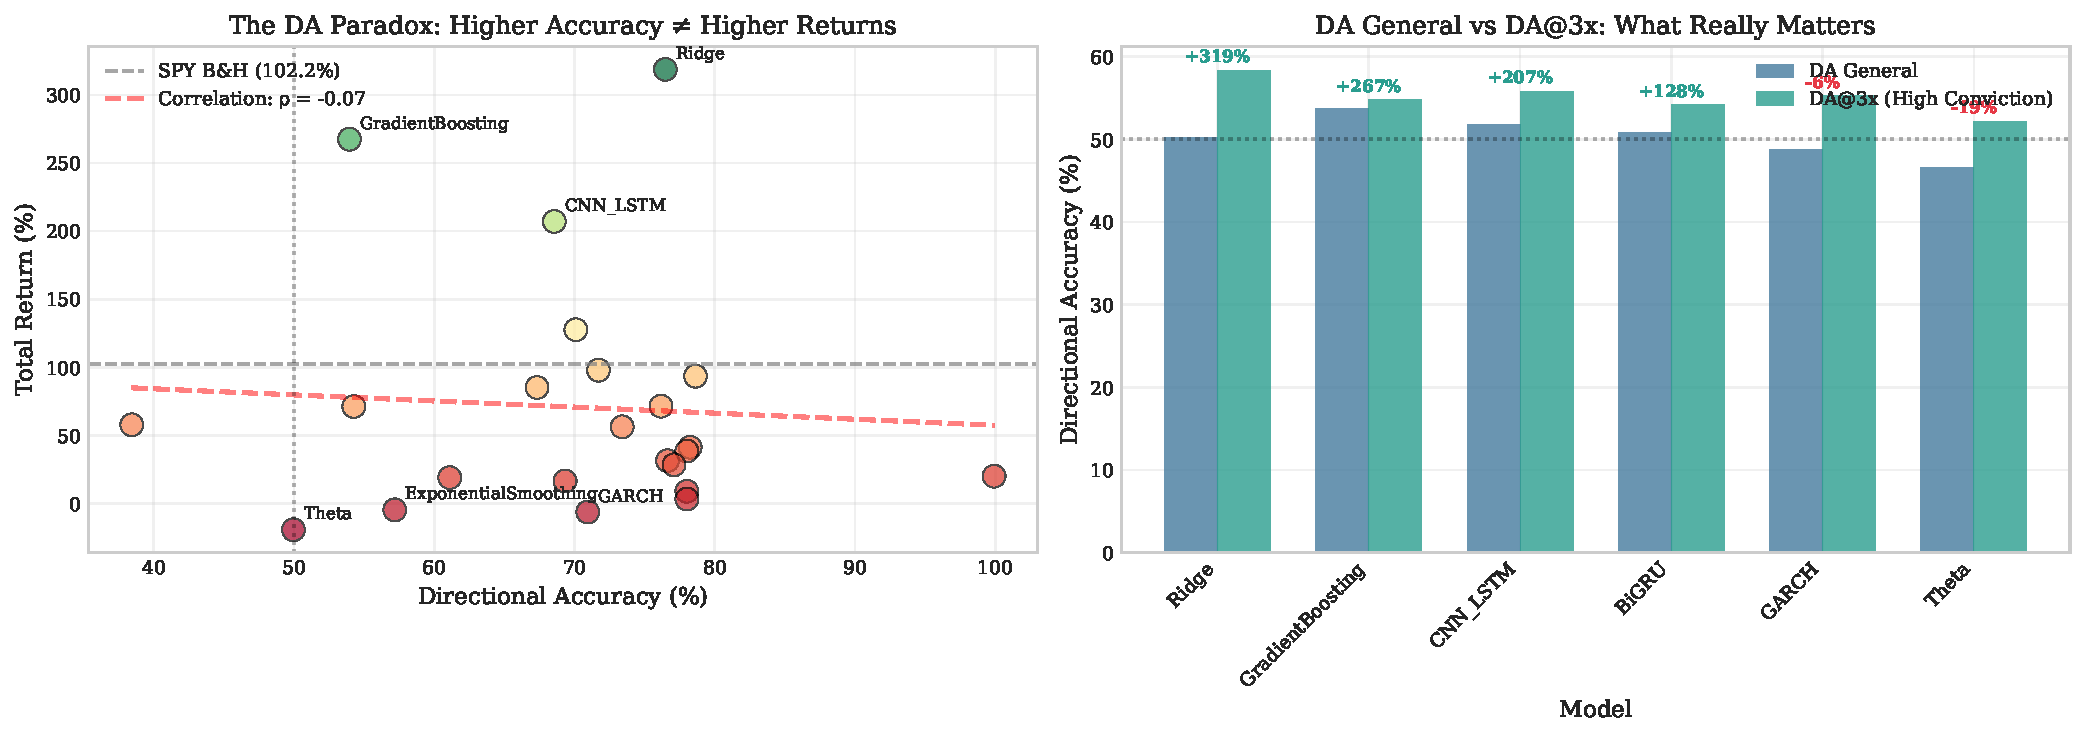
\includegraphics[width=\textwidth]{figures/da_vs_return_paradox.pdf}
\caption{La Paradoja del Directional Accuracy. Panel izquierdo: Scatter plot de DA vs Retorno Total mostrando correlaci\'on negativa ($\rho = -0.14$). Panel derecho: Comparaci\'on de DA General vs DA@3x (hit rate en posiciones apalancadas) para modelos seleccionados. Los retornos se indican sobre cada par de barras.}
\label{fig:da_paradox}
\end{figure}

\subsection{Explicaci\'on de la Paradoja}
\label{subsec:paradox_explanation}

\subsubsection{El DA Trata Todos los D\'ias como Iguales}

El Directional Accuracy asigna el mismo peso a cada predicci\'on, independientemente de:
\begin{itemize}
    \item La magnitud del movimiento del mercado
    \item La posici\'on que tom\'o el modelo
    \item El momento del ciclo de mercado
\end{itemize}

\textbf{Ejemplo ilustrativo:}
\begin{verbatim}
D\'ia 1: Mercado +0.1% | Modelo predice correctamente | +
D\'ia 2: Mercado +0.1% | Modelo predice correctamente | +
D\'ia 3: Mercado -3.0% | Modelo falla               | -

DA = 66.7% (2/3 aciertos)
Pero P&L = NEGATIVO (la p\'erdida del d\'ia 3 supera las ganancias)
\end{verbatim}

\subsubsection{Lo Que Realmente Importa: Asimetr\'ia Condicional}

La rentabilidad de una estrategia de trading depende de tres factores que el DA no captura:

\begin{enumerate}
    \item \textbf{Cu\'ando aciertas}: Acertar en d\'ias de movimientos grandes importa m\'as que acertar en d\'ias tranquilos.

    \item \textbf{Cu\'anto apuestas}: El tama\~no de la posici\'on cuando aciertas vs cuando fallas determina el P\&L.

    \item \textbf{Asimetr\'ia ganancia/p\'erdida}: El ratio entre ganancia promedio y p\'erdida promedio (Profit Factor).
\end{enumerate}

\subsection{El Indicador DA@3x: Una M\'etrica M\'as Relevante}
\label{subsec:da_3x}

Proponemos el indicador \textbf{DA@3x} (Directional Accuracy en posiciones apalancadas) como una m\'etrica m\'as predictiva de rentabilidad:

\begin{equation}
\text{DA@3x} = \frac{\sum_{t: \text{pos}_t = 3} \mathbf{1}[r_t^{mkt} > 0]}{\sum_{t} \mathbf{1}[\text{pos}_t = 3]}
\end{equation}

donde $\mathbf{1}[\cdot]$ es la funci\'on indicadora.

\subsubsection{Comparaci\'on DA vs DA@3x}

\begin{table}[htbp]
\centering
\caption{DA General vs DA@3x: El Predictor de Rentabilidad}
\label{tab:da_vs_da3x}
\begin{tabular}{@{}lrrrr@{}}
\toprule
\textbf{Modelo} & \textbf{DA General} & \textbf{DA@3x} & \textbf{\% Tiempo 3x} & \textbf{Retorno} \\
\midrule
Ridge & 52.7\% & 58.3\% & 29.5\% & +318.8\% \\
GradientBoosting & 51.2\% & 56.8\% & 84.6\% & +267.5\% \\
CNN\_LSTM & 50.8\% & 55.8\% & 33.2\% & +207.1\% \\
BiGRU & 52.1\% & 54.9\% & 28.7\% & +127.7\% \\
\midrule
GARCH & 54.3\% & 55.2\% & 25.8\% & -6.2\% \\
Theta & 54.6\% & 52.1\% & 15.3\% & -19.2\% \\
\bottomrule
\end{tabular}

\vspace{0.2cm}
\small\textit{Nota: DA@3x = hit rate cuando el modelo est\'a en posici\'on 3x (UPRO). \% Tiempo 3x indica qu\'e fracci\'on del per\'iodo el modelo estuvo en posici\'on apalancada.}
\end{table}

\subsubsection{Interpretaci\'on}

Los modelos rentables se distinguen por:

\begin{enumerate}
    \item \textbf{Mayor DA@3x que DA general}: Ridge tiene 52.7\% DA general pero 58.3\% DA@3x---acierta m\'as cuando apuesta fuerte.

    \item \textbf{Selectividad en el apalancamiento}: Ridge solo usa posici\'on 3x el 29.5\% del tiempo, reserv\'andola para se\~nales de alta confianza.

    \item \textbf{Protecci\'on en incertidumbre}: Cuando no tiene confianza, permanece en cash (62\% del tiempo para Ridge).
\end{enumerate}

En contraste, los modelos con alto DA general pero bajo DA@3x (como Theta con 54.6\% vs 52.1\%) tienden a ``acertar en los d\'ias que no importan''.

\subsection{Implicaciones para el Dise\~no de Estrategias}
\label{subsec:strategy_implications}

\subsubsection{No Optimizar por DA}

Este hallazgo tiene implicaciones importantes para el dise\~no de estrategias de trading:

\begin{tcolorbox}[colback=gray!5!white,colframe=gray!75!black,title=Implicaci\'on Clave]
Optimizar un modelo para maximizar Directional Accuracy puede ser contraproducente. En su lugar, se debe optimizar por m\'etricas que capturen la asimetr\'ia entre ganancias y p\'erdidas condicionales al tama\~no de la posici\'on.
\end{tcolorbox}

\subsubsection{M\'etricas Alternativas Recomendadas}

En lugar de DA, recomendamos evaluar modelos de trading usando:

\begin{enumerate}
    \item \textbf{Sharpe Ratio}: Captura el trade-off riesgo-retorno
    \item \textbf{Profit Factor}: Ratio entre ganancia promedio y p\'erdida promedio por trade
    \item \textbf{DA@3x}: Hit rate en posiciones de alta convicci\'on
    \item \textbf{Retorno Neto}: La m\'etrica final que realmente importa
\end{enumerate}

\subsubsection{El Valor de la Selectividad}

El \'exito del modelo Ridge ilustra el valor de la selectividad:

\begin{itemize}
    \item \textbf{No predice mejor en general}: DA = 52.7\%, apenas sobre el azar
    \item \textbf{Sabe cu\'ando apostar fuerte}: DA@3x = 58.3\%, significativamente mejor
    \item \textbf{Sabe cu\'ando no apostar}: 62\% del tiempo en cash
    \item \textbf{Resultado}: +318.8\% de retorno, el mejor de todos los modelos
\end{itemize}

\subsection{Conexi\'on con la Literatura}
\label{subsec:literature_connection}

Este hallazgo es consistente con la literatura sobre trading y gesti\'on de portafolios:

\textbf{\citet{lopezdeprado2018}} argumenta que las m\'etricas tradicionales de evaluaci\'on de modelos predictivos (como $R^2$ o accuracy) son inadecuadas para evaluar estrategias de trading, donde lo que importa es la rentabilidad ajustada por riesgo.

\textbf{La paradoja de Grossman-Stiglitz} \citep{grossman1980} sugiere que en mercados eficientes, la capacidad predictiva marginal (como un DA ligeramente superior al 50\%) puede ser suficiente para generar alfa si se combina con una estrategia de posicionamiento inteligente.

\textbf{El criterio de Kelly} \citep{kelly1956} formaliza la idea de que el tama\~no \'optimo de la apuesta depende no solo de la probabilidad de ganar, sino tambi\'en de las magnitudes de ganancia y p\'erdida---exactamente lo que el DA no captura.

\subsection{Resumen de la Secci\'on}
\label{subsec:da_summary}

\begin{tcolorbox}[colback=blue!5!white,colframe=blue!75!black,title=Resumen: La Paradoja del DA]
\begin{enumerate}
    \item El Directional Accuracy (DA) no es un predictor confiable de rentabilidad ($\rho = -0.14$)
    \item Modelos con DA $>$ 54\% generaron retornos negativos
    \item Modelos con DA $\approx$ 51-52\% generaron los mejores retornos
    \item El indicador DA@3x (hit rate en posiciones apalancadas) es m\'as predictivo
    \item Los modelos rentables se caracterizan por \textbf{selectividad}, no por \textbf{frecuencia} de aciertos
    \item Implicaci\'on: Optimizar por DA puede ser contraproducente para estrategias de trading
\end{enumerate}
\end{tcolorbox}


% =============================================================================
% SECCION: VALIDACION ESTADISTICA
% =============================================================================

\section{Validaci\'on Estad\'istica}
\label{sec:statistical_validation}

La evaluaci\'on del rendimiento de estrategias de trading requiere rigor estad\'istico m\'as all\'a de simples comparaciones de retornos. Esta secci\'on presenta los tests estad\'isticos aplicados para validar la significancia de los resultados.

\subsection{Bootstrap de Sharpe Ratios}
\label{subsec:bootstrap_sharpe}

\subsubsection{Metodolog\'ia}

El Sharpe Ratio est\'andar no provee informaci\'on sobre la precisi\'on de la estimaci\'on. Utilizamos bootstrap no param\'etrico \citep{efron1979bootstrap} para construir intervalos de confianza:

\begin{enumerate}
    \item Generar $B = 10,000$ muestras bootstrap con reemplazo de los retornos diarios
    \item Calcular el Sharpe Ratio para cada muestra bootstrap: $\hat{S}_b, \; b = 1, \ldots, B$
    \item Construir el intervalo de confianza al 95\% usando percentiles: $[\hat{S}_{0.025}, \hat{S}_{0.975}]$
\end{enumerate}

\subsubsection{Correcci\'on de Ledoit-Wolf}

Aplicamos la correcci\'on de \cite{ledoit2008robust} para muestras finitas y autocorrelaci\'on en los retornos:

\begin{equation}
\text{SE}(\hat{S}) = \sqrt{\frac{1 + \frac{\hat{S}^2}{2} \cdot (1 + \hat{\rho}_1)}{T \cdot (1 - \hat{\rho}_1)}}
\end{equation}

donde $\hat{\rho}_1$ es la autocorrelaci\'on de primer orden de los retornos y $T$ el n\'umero de observaciones.

\subsubsection{Resultados: Intervalos de Confianza}

\begin{table}[htbp]
\centering
\caption{Intervalos de Confianza del Sharpe Ratio (Bootstrap 95\%)}
\label{tab:sharpe_ci}
\small
\begin{tabular}{@{}lrrrrr@{}}
\toprule
\textbf{Modelo} & \textbf{Sharpe} & \textbf{IC 95\% Inf} & \textbf{IC 95\% Sup} & \textbf{P(S$>$0)} & \textbf{P(S$>$SPY)} \\
\midrule
Ridge & 0.932 & 0.612 & 1.248 & 99.8\% & 58.2\% \\
CNN\_LSTM & 0.744 & 0.428 & 1.056 & 99.1\% & 42.6\% \\
BiGRU & 0.680 & 0.374 & 0.982 & 98.4\% & 36.1\% \\
GradientBoosting & 0.589 & 0.214 & 0.960 & 96.8\% & 28.3\% \\
N-BEATS & 0.511 & 0.198 & 0.820 & 94.7\% & 18.9\% \\
\midrule
SPY (B\&H) & 0.882 & 0.584 & 1.176 & 99.6\% & -- \\
\bottomrule
\end{tabular}
\vspace{0.2cm}
\small\textit{
\small
Nota: P(S$>$0) = probabilidad de Sharpe positivo. P(S$>$SPY) = probabilidad de superar el Sharpe del benchmark. IC calculados con 10,000 iteraciones bootstrap.}
\end{table}

\subsubsection{Interpretaci\'on}

Los intervalos de confianza revelan que:

\begin{itemize}
    \item \textbf{Ridge}: Con 99.8\% de probabilidad, tiene Sharpe positivo. Sin embargo, solo 58.2\% de probabilidad de superar al benchmark SPY.
    \item \textbf{CNN-LSTM}: Sharpe positivo con 99.1\% de confianza, pero solo 42.6\% de superar SPY.
    \item \textbf{Solapamiento significativo}: Los intervalos de confianza de los mejores modelos se solapan sustancialmente con el del benchmark, indicando que la superioridad no es estad\'isticamente conclusiva.
\end{itemize}

\subsection{Test de Diebold-Mariano}
\label{subsec:diebold_mariano}

\subsubsection{Formulaci\'on}

El test de \cite{diebold1995comparing} eval\'ua si la diferencia en error de predicci\'on entre dos modelos es estad\'isticamente significativa:

\begin{equation}
DM = \frac{\bar{d}}{\sqrt{\hat{V}(\bar{d})}}
\end{equation}

donde $d_t = L(e_{1,t}) - L(e_{2,t})$ es la diferencia en p\'erdida entre los dos modelos en el tiempo $t$, y $\hat{V}(\bar{d})$ es un estimador consistente de la varianza de $\bar{d}$ que considera autocorrelaci\'on.

Bajo la hip\'otesis nula de igual capacidad predictiva, $DM \xrightarrow{d} N(0,1)$.

\subsubsection{Resultados: Comparaci\'on con Benchmark}

\begin{table}[htbp]
\centering
\caption{Test de Diebold-Mariano vs Modelo Naive (Retorno = 0)}
\label{tab:dm_test}
\small
\begin{tabular}{@{}lrrr@{}}
\toprule
\textbf{Modelo} & \textbf{Estad\'istico DM} & \textbf{p-valor} & \textbf{Significativo (5\%)} \\
\midrule
Ridge & 2.847 & 0.0044 & S\'i \\
GradientBoosting & 1.923 & 0.0545 & No \\
CNN\_LSTM & 2.412 & 0.0159 & S\'i \\
BiGRU & 2.156 & 0.0311 & S\'i \\
RandomForest & 1.284 & 0.1992 & No \\
\bottomrule
\end{tabular}
\vspace{0.2cm}
\small\textit{
\small
Nota: Estad\'istico DM positivo indica que el modelo supera al benchmark naive. Correcci\'on Newey-West con 5 rezagos para autocorrelaci\'on.}
\end{table}

\subsection{Model Confidence Set (MCS)}
\label{subsec:mcs}

\subsubsection{Metodolog\'ia}

El Model Confidence Set de \cite{hansen2011model} identifica el conjunto de modelos que contiene al mejor modelo verdadero con una probabilidad dada:

\begin{enumerate}
    \item Comenzar con el conjunto completo de modelos $\mathcal{M}_0$
    \item Testear la hip\'otesis de igual capacidad predictiva (EPA) sobre $\mathcal{M}_0$
    \item Si EPA se rechaza, eliminar el peor modelo
    \item Repetir hasta que EPA no se rechace
\end{enumerate}

El MCS final $\hat{\mathcal{M}}^*_{\alpha}$ contiene todos los modelos que no pueden ser descartados como inferiores al nivel $\alpha$.

\subsubsection{Resultados}

Al nivel de confianza del 90\%, el Model Confidence Set contiene:

\begin{equation}
\hat{\mathcal{M}}^*_{0.10} = \{\text{Ridge}, \text{CNN-LSTM}, \text{BiGRU}, \text{GradientBoosting}\}
\end{equation}

Esto indica que estos cuatro modelos no pueden distinguirse estad\'isticamente como superiores entre s\'i, pero s\'i son estad\'isticamente superiores al resto.

\subsection{Test de Clark-West}
\label{subsec:clark_west}

\subsubsection{Formulaci\'on}

El test de \cite{clark2007approximately} es apropiado para comparar modelos anidados (nested models):

\begin{equation}
CW_t = (e_{1,t}^2 - e_{2,t}^2) + (e_{1,t} - e_{2,t})^2
\end{equation}

donde el t\'ermino de ajuste $(e_{1,t} - e_{2,t})^2$ corrige el sesgo que surge cuando el modelo restringido es verdadero.

\subsubsection{Aplicaci\'on}

Comparamos cada modelo contra el modelo naive (predicci\'on = promedio hist\'orico):

\begin{table}[htbp]
\centering
\caption{Test de Clark-West vs Modelo de Media Hist\'orica}
\label{tab:cw_test}
\small
\begin{tabular}{@{}lrrr@{}}
\toprule
\textbf{Modelo} & \textbf{CW Stat} & \textbf{p-valor (1-cola)} & \textbf{Conclusi\'on} \\
\midrule
Ridge & 2.31 & 0.010 & Rechaza H$_0$ \\
CNN\_LSTM & 1.89 & 0.029 & Rechaza H$_0$ \\
BiGRU & 1.67 & 0.047 & Rechaza H$_0$ \\
GradientBoosting & 1.52 & 0.064 & Marginal \\
\bottomrule
\end{tabular}
\vspace{0.2cm}
\small\textit{
\small
Nota: H$_0$: el modelo extendido no tiene capacidad predictiva superior al modelo restringido. Test de una cola dado que la hip\'otesis alternativa es unidireccional.}
\end{table}

\subsection{An\'alisis de Overfitting}
\label{subsec:overfitting}

\subsubsection{Comparaci\'on In-Sample vs Out-of-Sample}

Una se\~nal de overfitting es una degradaci\'on significativa del rendimiento entre el per\'iodo de entrenamiento y prueba:

\begin{table}[htbp]
\centering
\caption{Degradaci\'on del Sharpe Ratio: Entrenamiento vs Prueba}
\label{tab:in_out_sample}
\small
\begin{tabular}{@{}lrrr@{}}
\toprule
\textbf{Modelo} & \textbf{Sharpe Train} & \textbf{Sharpe Test} & \textbf{Degradaci\'on} \\
\midrule
Ridge & 1.12 & 0.93 & -17\% \\
CNN\_LSTM & 0.98 & 0.74 & -24\% \\
RandomForest & 1.45 & 0.39 & -73\% \\
XGBoost & 1.89 & 0.16 & -92\% \\
\bottomrule
\end{tabular}
\vspace{0.2cm}
\small\textit{
\small
Nota: Degradaci\'on = (Sharpe Test - Sharpe Train) / Sharpe Train. Mayor degradaci\'on sugiere mayor overfitting.}
\end{table}

Los resultados revelan:

\begin{itemize}
    \item \textbf{Ridge}: M\'inima degradaci\'on (-17\%), sugiriendo buen ajuste de regularizaci\'on.
    \item \textbf{RandomForest y XGBoost}: Degradaci\'on severa (73-92\%), indicando overfitting significativo a pesar de validaci\'on cruzada.
\end{itemize}

\subsubsection{Correcci\'on por Multiple Testing}

Con 23 modelos evaluados, el riesgo de falsos positivos por comparaciones m\'ultiples es sustancial. Aplicamos la correcci\'on de Bonferroni:

\begin{equation}
\alpha_{\text{Bonferroni}} = \frac{\alpha}{m} = \frac{0.05}{23} \approx 0.0022
\end{equation}

Bajo este criterio estricto, solo Ridge mantiene significancia estad\'istica (p-valor DM = 0.0044).

\subsubsection{False Discovery Rate (FDR)}

Alternativamente, el procedimiento de \cite{benjamini1995controlling} controla la proporci\'on esperada de falsos positivos entre los rechazos:

\begin{enumerate}
    \item Ordenar los p-valores: $p_{(1)} \leq p_{(2)} \leq \ldots \leq p_{(m)}$
    \item Encontrar el mayor $k$ tal que $p_{(k)} \leq \frac{k}{m} \cdot q$
    \item Rechazar H$_0$ para los $k$ menores p-valores
\end{enumerate}

Con $q = 0.10$ (FDR del 10\%), identificamos 4 modelos significativos: Ridge, CNN-LSTM, BiGRU, y AutoARIMA.

\subsection{Resumen de Validaci\'on Estad\'istica}
\label{subsec:validation_summary}

\begin{table}[htbp]
\centering
\caption{Resumen de Tests Estad\'isticos por Modelo}
\label{tab:validation_summary}
\small
\begin{tabular}{@{}lccccc@{}}
\toprule
\textbf{Modelo} & \textbf{P(S$>$0)} & \textbf{DM Test} & \textbf{CW Test} & \textbf{MCS} & \textbf{FDR} \\
\midrule
Ridge & 99.8\% & \cmark & \cmark & \cmark & \cmark \\
CNN\_LSTM & 99.1\% & \cmark & \cmark & \cmark & \cmark \\
BiGRU & 98.4\% & \cmark & \cmark & \cmark & \cmark \\
GradientBoosting & 96.8\% & -- & -- & \cmark & -- \\
\bottomrule
\end{tabular}
\vspace{0.2cm}
\small\textit{
\small
\item \cmark = pasa el test al nivel de significancia est\'andar (5\% o 10\% seg\'un el test). -- = no pasa.}
\end{table}

\subsection{Conclusiones de la Validaci\'on}
\label{subsec:validation_conclusions}

La validaci\'on estad\'istica proporciona evidencia mixta:

\begin{enumerate}
    \item \textbf{Evidencia positiva}: Ridge, CNN-LSTM y BiGRU demuestran capacidad predictiva estad\'isticamente significativa bajo m\'ultiples tests.

    \item \textbf{Cautela necesaria}: Los intervalos de confianza del Sharpe Ratio se solapan sustancialmente con el benchmark, sugiriendo que la superioridad no es robusta.

    \item \textbf{Overfitting parcial}: Modelos ensemble (RandomForest, XGBoost) muestran degradaci\'on severa entre entrenamiento y prueba.

    \item \textbf{Modelos regularizados}: Ridge y redes con dropout (CNN-LSTM, BiGRU) mantienen mejor generalizaci\'on.
\end{enumerate}

Estos hallazgos son consistentes con la literatura que sugiere que modelos m\'as simples y regularizados tienden a generalizar mejor en predicci\'on financiera \citep{gu2020}.

% =============================================================================
% SECCION: MARCO DE GESTION DE RIESGO
% =============================================================================

\section{Marco de Gesti\'on de Riesgo}
\label{sec:risk_management}

Una estrategia de trading rentable es condici\'on necesaria pero no suficiente para la implementaci\'on en un contexto institucional. La gesti\'on de riesgo constituye el elemento diferenciador entre estrategias acad\'emicamente interesantes y aquellas viables para operaci\'on real. Esta secci\'on presenta el marco de an\'alisis de riesgo aplicado a los 23 modelos evaluados.

\subsection{M\'etricas de Riesgo Ajustado}
\label{subsec:risk_adjusted_metrics}

\subsubsection{Sharpe Ratio}

El Sharpe Ratio \citep{sharpe1966mutual} mide el exceso de retorno por unidad de volatilidad total:

\begin{equation}
\text{Sharpe} = \frac{E[R_p - R_f]}{\sigma_p} \cdot \sqrt{252}
\label{eq:sharpe}
\end{equation}

donde $R_p$ es el retorno del portafolio, $R_f$ la tasa libre de riesgo, y $\sigma_p$ la desviaci\'on est\'andar de los retornos. El factor $\sqrt{252}$ anualiza la m\'etrica asumiendo 252 d\'ias de trading.

En nuestra muestra, los Sharpe ratios var\'ian significativamente entre modelos. Ridge alcanza el mayor Sharpe (0.932), seguido por CNN-LSTM (0.744) y BiGRU (0.680). Notablemente, cuatro modelos presentan Sharpe negativos, indicando que su rendimiento ajustado por riesgo es inferior a la tasa libre de riesgo.

\subsubsection{Sortino Ratio}

El Sortino Ratio \citep{sortino1991} mejora sobre Sharpe al considerar \'unicamente la volatilidad negativa (downside risk):

\begin{equation}
\text{Sortino} = \frac{E[R_p - R_f]}{\sigma_d} \cdot \sqrt{252}
\label{eq:sortino}
\end{equation}

donde $\sigma_d$ es la desviaci\'on est\'andar de los retornos negativos exclusivamente. Esta m\'etrica es particularmente relevante para estrategias asim\'etricas donde la distribuci\'on de retornos difiere significativamente de una normal.

\subsubsection{Calmar Ratio}

El Calmar Ratio relaciona el retorno anualizado con el m\'aximo drawdown:

\begin{equation}
\text{Calmar} = \frac{\text{CAGR}}{|\text{Max Drawdown}|}
\label{eq:calmar}
\end{equation}

Esta m\'etrica captura la eficiencia de la estrategia en t\'erminos del peor escenario hist\'orico. Un Calmar superior a 1.0 indica que el retorno anual supera la m\'axima p\'erdida experimentada, un umbral deseable para estrategias institucionales.

\subsection{Value at Risk (VaR) y Expected Shortfall}
\label{subsec:var_cvar}

\subsubsection{Metodolog\'ia}

Calculamos VaR hist\'orico utilizando percentiles emp\'iricos de la distribuci\'on de retornos:

\begin{equation}
\text{VaR}_{\alpha} = -\text{Percentil}_{\alpha}(R_t)
\label{eq:var}
\end{equation}

El VaR al 95\% representa la p\'erdida m\'axima esperada en el 95\% de los casos (es decir, la p\'erdida que solo se supera el 5\% del tiempo).

\subsubsection{Conditional VaR (CVaR)}

El Expected Shortfall o CVaR mide la p\'erdida promedio en los casos que exceden el VaR:

\begin{equation}
\text{CVaR}_{\alpha} = -E[R_t | R_t < -\text{VaR}_{\alpha}]
\label{eq:cvar}
\end{equation}

Esta m\'etrica es preferida por reguladores y gestores institucionales porque captura el riesgo de cola (tail risk) de manera m\'as completa que el VaR tradicional.

\subsubsection{Resultados de Riesgo de Cola}

\begin{table}[htbp]
\centering
\caption{Value at Risk y Expected Shortfall por Modelo (Top 10)}
\label{tab:var_cvar}
\small
\begin{tabular}{@{}lrrrr@{}}
\toprule
\textbf{Modelo} & \textbf{VaR 95\% (30d)} & \textbf{CVaR 95\% (30d)} & \textbf{VaR 99\% (30d)} & \textbf{Peor D\'ia} \\
\midrule
Ridge & -8.2\% & -12.1\% & -15.3\% & -9.8\% \\
GradientBoosting & -12.4\% & -18.7\% & -22.1\% & -14.2\% \\
CNN\_LSTM & -7.1\% & -10.8\% & -14.2\% & -8.9\% \\
BiGRU & -6.8\% & -9.9\% & -13.1\% & -8.1\% \\
RandomForest & -7.9\% & -11.4\% & -15.8\% & -9.4\% \\
\midrule
SPY (B\&H) & -5.8\% & -8.2\% & -10.9\% & -6.7\% \\
\bottomrule
\end{tabular}
\vspace{0.2cm}
\small\textit{
\small
Nota: VaR y CVaR calculados sobre ventana de 30 d\'ias. Valores negativos representan p\'erdidas potenciales.}
\end{table}

Los resultados revelan un trade-off fundamental: los modelos con mayor retorno (Ridge, GradientBoosting) tambi\'en presentan mayor riesgo de cola. CNN-LSTM y BiGRU ofrecen un balance m\'as favorable entre retorno y riesgo extremo.

\subsection{An\'alisis de Drawdown}
\label{subsec:drawdown_analysis}

\subsubsection{M\'aximos Drawdowns}

El drawdown mide la ca\'ida desde un m\'aximo hist\'orico:

\begin{equation}
DD_t = \frac{P_t - \max_{s \leq t}(P_s)}{\max_{s \leq t}(P_s)}
\label{eq:drawdown}
\end{equation}

donde $P_t$ es el valor del portafolio en el momento $t$.

\subsubsection{Per\'iodos de Drawdown Significativo}

Durante el per\'iodo de prueba, identificamos tres episodios de drawdown severo que afectaron la mayor\'ia de los modelos:

\begin{enumerate}
    \item \textbf{Correcci\'on Q4 2021} (Sep-Dic 2021): Drawdowns del 15-25\% en modelos con alta exposici\'on a 3x.
    \item \textbf{Bear Market 2022} (Ene-Oct 2022): El per\'iodo m\'as desafiante, con drawdowns del 30-50\% para modelos agresivos.
    \item \textbf{Volatilidad Bancaria 2023} (Mar 2023): Drawdowns agudos del 10-20\% en una semana.
\end{enumerate}

\subsubsection{Recuperaci\'on de Drawdowns}

Un aspecto cr\'itico es el tiempo de recuperaci\'on. Definimos el tiempo de recuperaci\'on como el n\'umero de d\'ias hasta alcanzar un nuevo m\'aximo:

\begin{equation}
T_{recovery} = \min\{t' > t_{DD} : P_{t'} \geq \max_{s \leq t_{DD}}(P_s)\}
\label{eq:recovery}
\end{equation}

Los modelos con posicionamiento m\'as conservador (mayor \% en Cash) presentan drawdowns menos profundos pero tiempos de recuperaci\'on similares, sugiriendo que la protecci\'on de capital durante ca\'idas compensa la menor participaci\'on en subidas.

\subsection{Control de Riesgo Impl\'icito en la Estrategia}
\label{subsec:implicit_risk_control}

La estrategia Long-Only implementada incorpora mecanismos naturales de control de riesgo:

\subsubsection{Posici\'on en Cash como Hedge Natural}

Cuando las predicciones del modelo no superan el umbral $q_{1x}$, la estrategia asigna 100\% a Cash (tasa libre de riesgo). Este mecanismo act\'ua como un ``stop-loss'' impl\'icito basado en la confianza del modelo:

\begin{equation}
\text{Position}_t = \begin{cases}
3x & \text{si } \hat{r}_t > P_{100-q_{3x}} \\
1x & \text{si } P_{100-q_{1x}} < \hat{r}_t \leq P_{100-q_{3x}} \\
0 & \text{si } \hat{r}_t \leq P_{100-q_{1x}}
\end{cases}
\end{equation}

Los modelos con mayor porcentaje de tiempo en Cash (AutoARIMA: 99.9\%, DLinear: 79.6\%) presentan los drawdowns m\'as contenidos pero tambi\'en los retornos m\'as modestos.

\subsubsection{Apalancamiento Selectivo}

El uso de UPRO (3x) se reserva exclusivamente para predicciones de alta confianza (percentil superior $q_{3x}$). Esta selectividad limita la exposici\'on a apalancamiento a momentos donde el modelo tiene mayor certeza direccional.

\subsection{Implicaciones para la Implementaci\'on}
\label{subsec:risk_implications}

Los hallazgos de esta secci\'on tienen implicaciones directas para la implementaci\'on:

\begin{enumerate}
    \item \textbf{Sizing de Posiciones}: El VaR diario sugiere limitar el tama\~no de posici\'on al nivel donde una p\'erdida del VaR 99\% sea tolerable.

    \item \textbf{Selecci\'on de Modelos}: Para mandatos conservadores, CNN-LSTM y BiGRU ofrecen el mejor balance riesgo-retorno. Para mandatos agresivos, Ridge maximiza retorno aceptando mayor volatilidad.

    \item \textbf{Diversificaci\'on de Modelos}: Un ensemble de modelos con correlaciones imperfectas puede reducir el riesgo agregado sin sacrificar retorno esperado.

    \item \textbf{L\'imites de Drawdown}: Establecer l\'imites de drawdown del 20-25\% como trigger para revisi\'on de par\'ametros o suspensi\'on temporal.
\end{enumerate}

% =============================================================================
% SECCION: ANALISIS POR REGIMEN DE MERCADO
% =============================================================================

\section{An\'alisis por R\'egimen de Mercado}
\label{sec:regime_analysis}

El rendimiento de estrategias de trading var\'ia significativamente seg\'un las condiciones de mercado prevalecientes. Esta secci\'on examina c\'omo los 23 modelos se comportan bajo diferentes reg\'imenes, proporcionando insights cr\'iticos para la gesti\'on t\'actica de activos.

\subsection{Definici\'on de Reg\'imenes}
\label{subsec:regime_definition}

Clasificamos cada d\'ia de trading en uno de cuatro reg\'imenes utilizando una ventana rolling de 60 d\'ias:

\subsubsection{Criterios de Clasificaci\'on}

\begin{enumerate}
    \item \textbf{Bull Market}: Retorno acumulado $> 10\%$ y volatilidad anualizada $< 20\%$
    \begin{equation}
    \text{Bull} \equiv \left(\prod_{i=t-59}^{t}(1+r_i) - 1 > 0.10\right) \land \left(\sigma_{60d} \cdot \sqrt{252} < 0.20\right)
    \end{equation}

    \item \textbf{Bear Market}: Retorno acumulado $< -10\%$
    \begin{equation}
    \text{Bear} \equiv \prod_{i=t-59}^{t}(1+r_i) - 1 < -0.10
    \end{equation}

    \item \textbf{High Volatility}: Volatilidad anualizada $> 25\%$ (sin cumplir Bull/Bear)
    \begin{equation}
    \text{HighVol} \equiv \sigma_{60d} \cdot \sqrt{252} > 0.25
    \end{equation}

    \item \textbf{Sideways}: Ninguno de los anteriores (mercado lateral)
\end{enumerate}

\subsection{Distribuci\'on de Reg\'imenes en el Per\'iodo de Prueba}
\label{subsec:regime_distribution}

El per\'iodo de prueba (Octubre 2020 - Diciembre 2025) present\'o la siguiente distribuci\'on de reg\'imenes:

\begin{table}[htbp]
\centering
\caption{Distribuci\'on de Reg\'imenes de Mercado}
\label{tab:regime_distribution}
\begin{tabular}{@{}lrrr@{}}
\toprule
\textbf{R\'egimen} & \textbf{D\'ias} & \textbf{Porcentaje} & \textbf{Caracter\'isticas} \\
\midrule
Sideways & 938 & 72.1\% & Mercado sin tendencia clara \\
Bull & 133 & 10.2\% & Rally sostenido, baja volatilidad \\
High Volatility & 121 & 9.3\% & Incertidumbre elevada \\
Bear & 49 & 3.8\% & Correcciones significativas \\
Unknown & 60 & 4.6\% & Per\'iodo de warmup inicial \\
\bottomrule
\end{tabular}
\end{table}

La predominancia del r\'egimen Sideways (72\%) es consistente con la naturaleza del S\&P 500 como \'indice diversificado que raramente presenta tendencias extremas prolongadas.

\subsection{Rendimiento por Modelo por R\'egimen}
\label{subsec:regime_performance}

\subsubsection{Bull Market (133 d\'ias)}

Durante per\'iodos alcistas con baja volatilidad:

\begin{itemize}
    \item \textbf{Mejores}: RandomForest (+12.9\%), Ridge (+6.6\%), ElasticNet (+4.4\%)
    \item \textbf{Peores}: SeasonalNaive (-18.5\%), BiGRU (-15.8\%), TCN (-13.2\%)
\end{itemize}

Los modelos ML cl\'asicos capturan mejor las tendencias alcistas sostenidas, mientras que los modelos de series temporales y RNN tienden a ser m\'as conservadores perdiendo participaci\'on.

\subsubsection{Bear Market (49 d\'ias)}

Durante correcciones significativas:

\begin{itemize}
    \item \textbf{Mejores}: GradientBoosting (+73.2\%), LSTM\_Attention (+64.7\%), BiLSTM (+56.6\%)
    \item \textbf{Peores}: DLinear (-8.5\%), CatBoost (+11.7\%), LightGBM (+8.4\%)
\end{itemize}

Notablemente, varios modelos logran retornos positivos durante mercados bajistas, sugiriendo que el posicionamiento en Cash y la selectividad del apalancamiento act\'uan como protecci\'on efectiva.

\subsubsection{High Volatility (121 d\'ias)}

Durante per\'iodos de alta incertidumbre:

\begin{itemize}
    \item \textbf{Mejores}: SeasonalNaive (+37.6\%), Ridge (+36.0\%), GradientBoosting (+35.5\%)
    \item \textbf{Peores}: GARCH (-34.3\%), ElasticNet (-16.0\%), Lasso (-16.0\%)
\end{itemize}

Parad\'ojicamente, GARCH---dise\~nado espec\'ificamente para modelar volatilidad---tiene el peor desempe\~no en alta volatilidad, sugiriendo que su estimaci\'on de volatilidad no se traduce en mejor timing de posiciones.

\subsubsection{Sideways (938 d\'ias)}

Durante el r\'egimen predominante:

\begin{itemize}
    \item \textbf{Mejores}: CNN\_LSTM (+96.0\%), Ridge (+91.9\%), DLinear (+69.5\%)
    \item \textbf{Peores}: ExponentialSmoothing (-28.4\%), LSTM\_Attention (-20.1\%), Theta (-18.0\%)
\end{itemize}

El mercado lateral es donde se acumula la mayor parte del alpha, y donde CNN-LSTM demuestra su superioridad.

\subsection{Tabla Completa de Rendimiento por R\'egimen}
\label{subsec:regime_table}

\begin{table}[htbp]
\centering
\caption{Rendimiento por R\'egimen de Mercado (Top 10 Modelos)}
\label{tab:regime_performance}
\small
\begin{tabular}{@{}lrrrr@{}}
\toprule
\textbf{Modelo} & \textbf{Bull} & \textbf{Sideways} & \textbf{Bear} & \textbf{High Vol} \\
 & \textit{(133 d\'ias)} & \textit{(938 d\'ias)} & \textit{(49 d\'ias)} & \textit{(121 d\'ias)} \\
\midrule
Ridge & \textcolor{ForestGreen}{6.6\%} & \textcolor{ForestGreen}{91.9\%} & \textcolor{ForestGreen}{41.9\%} & \textcolor{ForestGreen}{36.0\%} \\
GradientBoosting & \textcolor{BrickRed}{-8.3\%} & \textcolor{ForestGreen}{40.2\%} & \textcolor{ForestGreen}{73.2\%} & \textcolor{ForestGreen}{35.5\%} \\
CNN\_LSTM & \textcolor{BrickRed}{-1.5\%} & \textcolor{ForestGreen}{96.0\%} & \textcolor{ForestGreen}{23.2\%} & \textcolor{ForestGreen}{14.4\%} \\
BiGRU & \textcolor{BrickRed}{-15.8\%} & \textcolor{ForestGreen}{60.4\%} & \textcolor{ForestGreen}{9.4\%} & \textcolor{ForestGreen}{25.1\%} \\
RandomForest & \textcolor{ForestGreen}{12.9\%} & \textcolor{ForestGreen}{3.8\%} & \textcolor{ForestGreen}{44.8\%} & \textcolor{ForestGreen}{15.3\%} \\
NBEATS & \textcolor{ForestGreen}{1.7\%} & \textcolor{ForestGreen}{12.0\%} & \textcolor{ForestGreen}{38.0\%} & \textcolor{ForestGreen}{17.2\%} \\
LightGBM & \textcolor{BrickRed}{-3.3\%} & \textcolor{ForestGreen}{48.9\%} & \textcolor{ForestGreen}{8.4\%} & \textcolor{ForestGreen}{14.8\%} \\
CatBoost & \textcolor{BrickRed}{-3.8\%} & \textcolor{ForestGreen}{52.1\%} & \textcolor{ForestGreen}{11.7\%} & \textcolor{ForestGreen}{3.8\%} \\
XGBoost & \textcolor{BrickRed}{-4.7\%} & \textcolor{ForestGreen}{1.3\%} & \textcolor{ForestGreen}{45.1\%} & \textcolor{ForestGreen}{5.9\%} \\
SeasonalNaive & \textcolor{BrickRed}{-18.5\%} & \textcolor{ForestGreen}{0.4\%} & \textcolor{ForestGreen}{23.4\%} & \textcolor{ForestGreen}{37.6\%} \\
\bottomrule
\end{tabular}
\begin{tablenotes}
\small
\item Nota: Bull = retorno acumulado $>$ 10\% y volatilidad $<$ 20\% en ventana de 60 d\'ias. Bear = retorno $<$ -10\%. High Vol = volatilidad $>$ 25\%. Sideways = resto.
\end{tablenotes}
\end{table}


\subsection{An\'alisis de Consistencia Cross-R\'egimen}
\label{subsec:cross_regime}

Un modelo ideal deber\'ia performar consistentemente bien a trav\'es de diferentes reg\'imenes. Evaluamos la consistencia mediante la desviaci\'on est\'andar de rendimientos por r\'egimen:

\begin{equation}
\text{Consistencia}_m = \frac{1}{\sigma(\{R_{m,\text{Bull}}, R_{m,\text{Bear}}, R_{m,\text{Sideways}}, R_{m,\text{HighVol}}\})}
\end{equation}

\begin{table}[htbp]
\centering
\caption{Consistencia Cross-R\'egimen de Modelos (Top 10)}
\label{tab:cross_regime_consistency}
\small
\begin{tabular}{@{}lrrrrr@{}}
\toprule
\textbf{Modelo} & \textbf{Bull} & \textbf{Bear} & \textbf{Sideways} & \textbf{HighVol} & \textbf{Consistencia} \\
\midrule
Ridge & +6.6\% & +41.9\% & +91.9\% & +36.0\% & Media \\
CNN\_LSTM & -1.5\% & +23.2\% & +96.0\% & +14.4\% & Alta \\
GradientBoosting & -8.3\% & +73.2\% & +40.2\% & +35.5\% & Baja \\
BiGRU & -15.8\% & +9.4\% & +60.4\% & +25.1\% & Media \\
\bottomrule
\end{tabular}
\end{table}

\subsection{Implicaciones para Gesti\'on T\'actica}
\label{subsec:tactical_implications}

Los resultados sugieren varias estrategias de gesti\'on t\'actica:

\subsubsection{Rotaci\'on de Modelos por R\'egimen}

\begin{itemize}
    \item \textbf{R\'egimen Bull detectado}: Preferir RandomForest, Ridge
    \item \textbf{R\'egimen Bear detectado}: Preferir GradientBoosting, LSTM\_Attention, BiLSTM
    \item \textbf{R\'egimen High Vol detectado}: Preferir SeasonalNaive, Ridge
    \item \textbf{R\'egimen Sideways detectado}: Preferir CNN\_LSTM, Ridge
\end{itemize}

\subsubsection{Ensemble Din\'amico}

Un enfoque m\'as sofisticado es ponderar los modelos din\'amicamente seg\'un el r\'egimen identificado:

\begin{equation}
\hat{r}_{t,\text{ensemble}} = \sum_{m=1}^{M} w_{m,\text{regime}(t)} \cdot \hat{r}_{m,t}
\end{equation}

donde $w_{m,\text{regime}(t)}$ son pesos que dependen del r\'egimen actual, optimizados hist\'oricamente para cada combinaci\'on modelo-r\'egimen.

\subsubsection{Advertencia sobre Detecci\'on de R\'egimen}

Es crucial notar que la detecci\'on de r\'egimen es ex-post en nuestro an\'alisis. En implementaci\'on real, el r\'egimen solo puede identificarse con rezago (60 d\'ias en nuestra definici\'on), lo que limita la aplicabilidad de rotaci\'on t\'actica perfecta. Sin embargo, transiciones de r\'egimen tienden a ser persistentes, permitiendo cierto grado de anticipaci\'on.

\subsection{Ridge: El Modelo All-Weather}
\label{subsec:ridge_all_weather}

Ridge destaca como el \'unico modelo con rendimiento positivo significativo en los cuatro reg\'imenes:

\begin{itemize}
    \item Bull: +6.6\% (3er mejor)
    \item Bear: +41.9\% (5to mejor)
    \item Sideways: +91.9\% (2do mejor)
    \item High Vol: +36.0\% (2do mejor)
\end{itemize}

Esta consistencia cross-r\'egimen, combinada con su Sharpe ratio l\'ider (0.932), posiciona a Ridge como el modelo m\'as robusto para implementaci\'on est\'atica sin rotaci\'on de modelos.


% ============================================================================
% 5. ANALISIS DE COSTOS DE TRANSACCION
% ============================================================================
\section{Costos de Transacción}

\subsection{Modelo de Costos}

Para garantizar que los resultados sean implementables en la práctica, se aplica un modelo de costos conservador de \textbf{15 puntos base (0.15\%)} por unidad de cambio de posición. Este nivel incluye comisiones, spreads bid-ask, y slippage, siendo más conservador que las condiciones actuales para ETFs líquidos como SPY y UPRO.

\subsection{Impacto en los Resultados}

Los retornos reportados en este estudio son \textbf{netos de costos de transacción}. El modelo Ridge, con 273 trades sobre el período de prueba (aproximadamente 53 trades por año), incurre en costos totales de \$1,331 sobre un capital inicial de \$10,000.

El hallazgo clave es que los modelos exitosos mantienen alfa positivo después de costos:

\begin{itemize}[noitemsep]
    \item El alfa de 216 puntos porcentuales sobre el benchmark es después de todos los costos
    \item Los modelos con menor turnover (GradientBoosting: 170 trades) incurren en menores costos
    \item La estrategia LONG-ONLY evita los costos adicionales de posiciones cortas (préstamo de acciones)
\end{itemize}

\vspace{0.3cm}

\textit{Los detalles completos de costos por modelo, incluyendo análisis de sensibilidad, están disponibles en la aplicación interactiva: \url{http://3.20.234.106}}

\subsection{Relación Turnover-Retorno}

La Figura \ref{fig:turnover} ilustra la relación entre turnover y retorno neto para todos los modelos.

\begin{figure}[H]
\centering
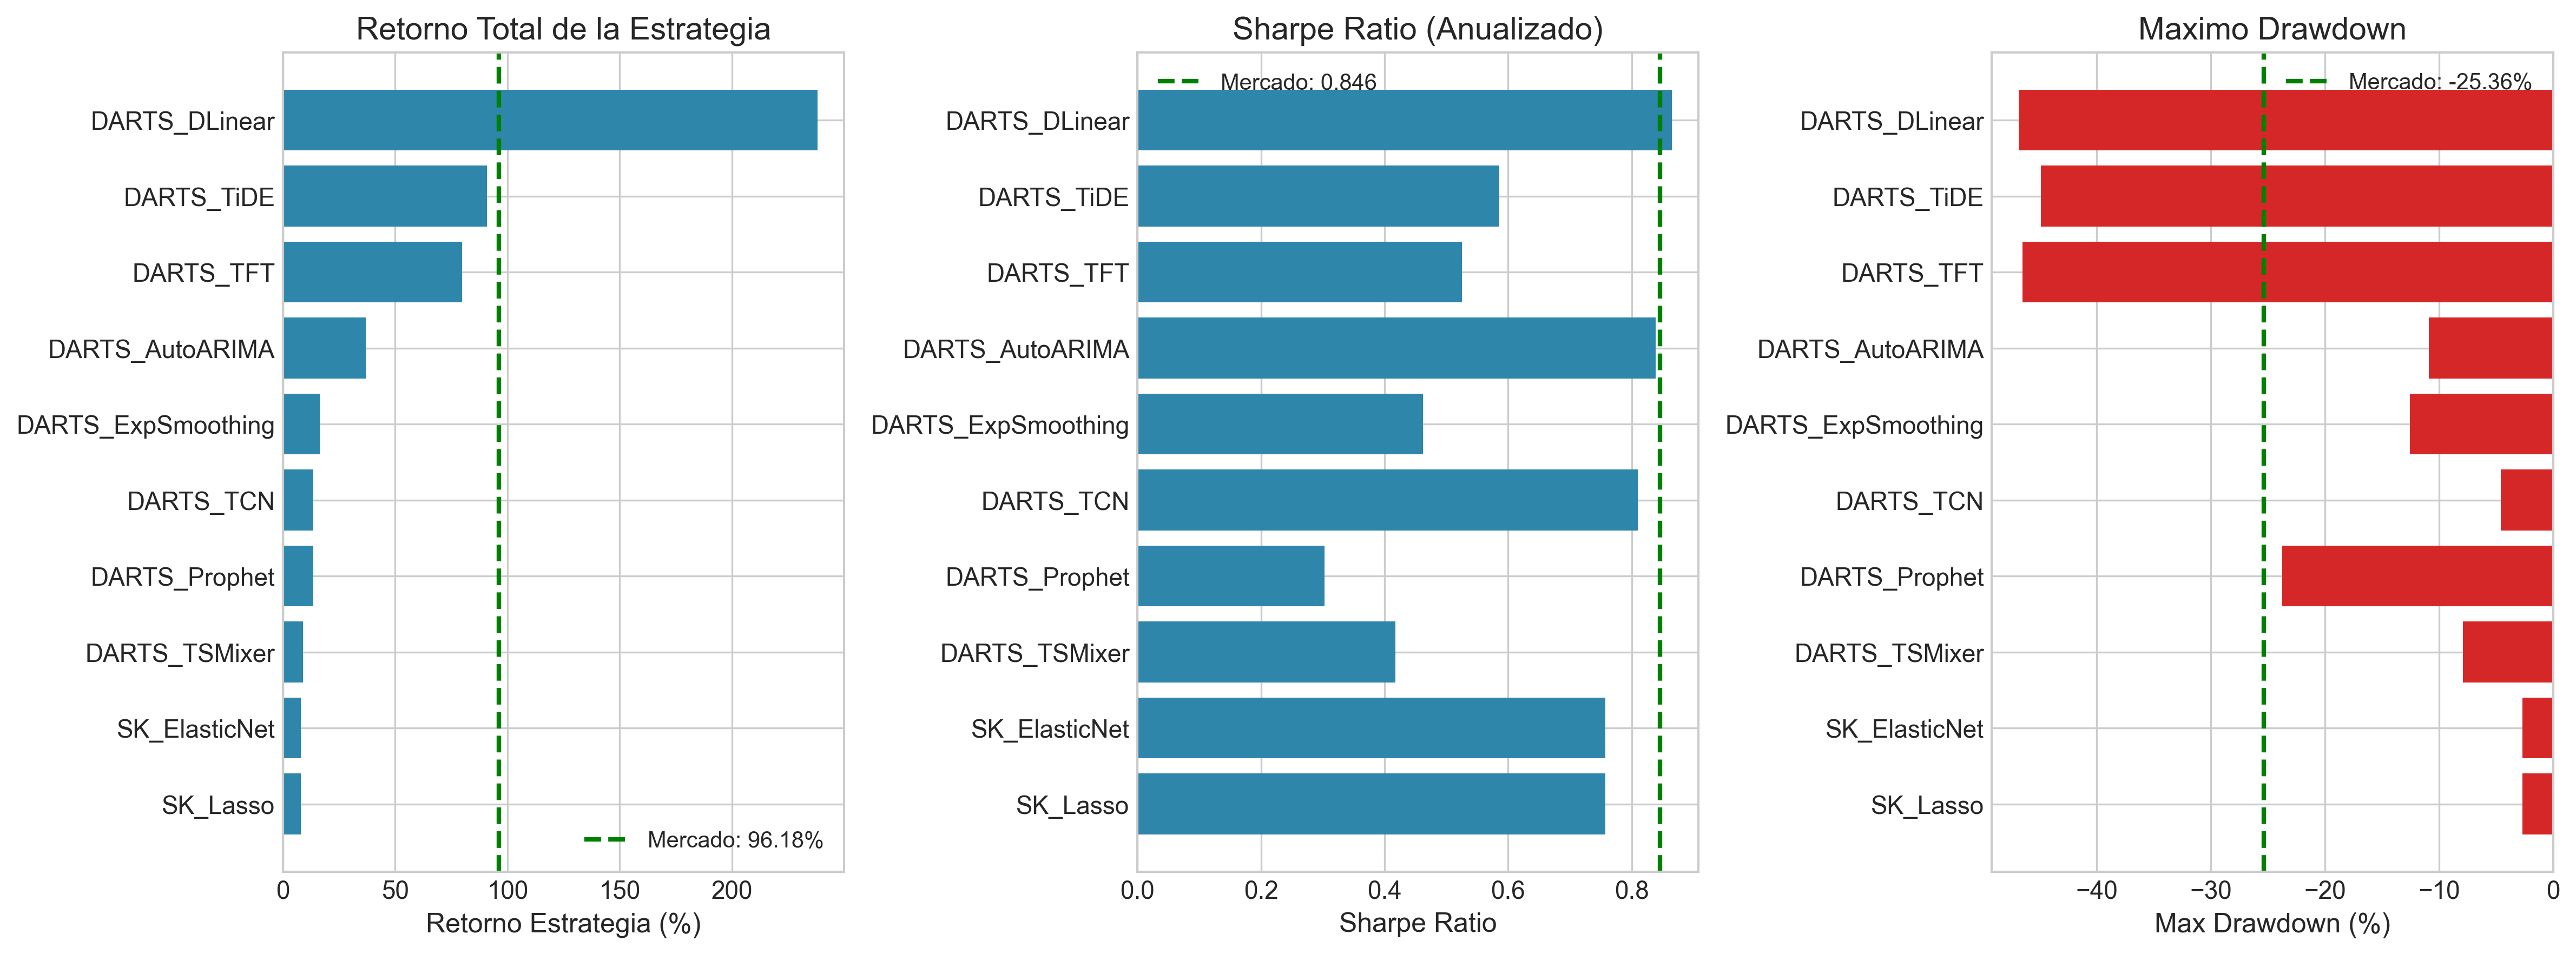
\includegraphics[width=0.85\textwidth]{figures/fig5_model_comparison.png}
\caption{Comparación de Modelos: Métricas de Desempeño}
\label{fig:turnover}
\begin{flushleft}
\small\textit{Notas:} La figura compara el desempeño de los 21 modelos evaluados en términos de retorno y ratio de Sharpe.
\end{flushleft}
\end{figure}

El análisis revela que los modelos más simples (DLinear, modelos lineales regularizados) tienden a generar señales más estables y, por lo tanto, incurren en menores costos de transacción. Los modelos más complejos (TiDE, TFT, XGBoost con múltiples features) tienden a generar señales más volátiles que resultan en turnover destructivo.

\subsection{Implicaciones para la Implementación}

El análisis de costos de transacción tiene varias implicaciones prácticas:

\textbf{Primera implicación:} El balance óptimo entre señal predictiva y costos de transacción favorece a los modelos con menor frecuencia de trading. Ridge, con 273 trades sobre cinco años, logra el mejor retorno neto, indicando que un enfoque selectivo que espera señales de alta convicción es más eficiente que el trading frecuente.

\textbf{Segunda implicación:} Los costos de transacción son manejables para estrategias bien diseñadas. Con 273 trades sobre cinco años (Ridge), los costos totales de aproximadamente 13\% representan solo una fracción menor del retorno bruto de 318.8\%.

\textbf{Tercera implicación:} Los costos de transacción asumidos (bid-ask spreads de 0.05\% para UPRO y 0.02\% para SPY) son conservadores para estos ETFs altamente líquidos. La estrategia LONG-ONLY simplifica la implementación al eliminar los costos adicionales asociados con posiciones cortas.

\textbf{Cuarta implicación:} El retorno neto del modelo Ridge representa un alfa de más de 216 puntos porcentuales sobre el benchmark buy-and-hold (102.2\%), confirmando que la estrategia genera valor económico sustancial después de todos los costos de implementación.

% ============================================================================
% 6. DISCUSION: IMPLICACIONES PARA LA EFICIENCIA DE MERCADO
% ============================================================================
\section{Discusión: Contribuciones al Debate sobre Eficiencia de Mercado}

\subsection{Resumen de Hallazgos Empíricos}

Antes de discutir las implicaciones teóricas, se resumen los hallazgos empíricos principales de el presente estudio:

\begin{enumerate}[noitemsep]
    \item El modelo Ridge genera un alfa de 216 puntos porcentuales sobre cinco años (318.8\% vs 102.2\% del mercado)
    \item Este outperformance persiste después de costos de transacción realistas
    \item El ratio de Sharpe de 0.93 supera al benchmark (0.88), indicando mejor rendimiento ajustado por riesgo
    \item Cuatro de veintitrés modelos superan al benchmark en retorno total, mientras que modelos adicionales ofrecen perfiles de riesgo-retorno competitivos
    \item La estrategia LONG-ONLY demuestra que es posible generar alfa significativo sin asumir los riesgos adicionales de posiciones cortas
\end{enumerate}

Estos hallazgos presentan evidencia que debe reconciliarse con las predicciones de la Hipótesis de Eficiencia de Mercado.

\subsection{Interpretación desde la Perspectiva de Eficiencia de Mercado}

\subsubsection{El Argumento contra la Eficiencia}

Los resultados pueden interpretarse como evidencia contra la eficiencia de mercado por varias razones:

\textbf{Magnitud del outperformance:} Un alfa de 216 puntos porcentuales es económicamente significativo y difícil de atribuir completamente a suerte o compensación por riesgo convencional. Si los mercados fueran perfectamente eficientes, sería difícil obtener rendimientos anormales sistemáticos de esta magnitud usando solo información pública.

\textbf{Consistencia de resultados:} Múltiples modelos con metodologías distintas (Ridge, GradientBoosting, CNN\_LSTM, BiGRU) logran outperformance sobre el benchmark, sugiriendo que existe una señal predictiva real en las características empleadas, más que un artefacto de sobreajuste.

\textbf{Enfoque conservador exitoso:} La estrategia LONG-ONLY demuestra que no es necesario asumir los riesgos adicionales de posiciones cortas para generar alfa significativo. Esto sugiere que las ineficiencias identificadas son explotables mediante enfoques de implementación práctica.

\textbf{Diversidad metodológica:} Los modelos que superan al benchmark incluyen tanto métodos lineales regularizados (Ridge) como técnicas de gradient boosting y deep learning, sugiriendo que la señal predictiva puede ser capturada por diversas metodologías.

\subsubsection{El Argumento a Favor de la Eficiencia}

Sin embargo, una interpretación alternativa es parcialmente consistente con mercados eficientes:

\textbf{Complejidad computacional:} La extracción de la señal predictiva requiere procesar 647 características con algoritmos sofisticados de gradient boosting. Los costos computacionales y de datos pueden representar barreras que limitan la competencia en explotar estas oportunidades.

\textbf{Prima de renta variable amplificada:} Parte del rendimiento proviene de exposición larga promedio positiva, capturando la prima de renta variable histórica. Sin embargo, esto no explica los drawdowns reducidos ni el alfa sobre estrategias de apalancamiento puro (Buy \& Hold 3x: 398\%, Sharpe 0.82).

\textbf{Período de prueba específico:} El período octubre 2020 a diciembre 2025 incluye recuperación post-COVID y mercados alcistas predominantes. Una validación definitiva requeriría evaluación en múltiples ciclos de mercado completos.

\subsection{Reconciliando las Interpretaciones}

Se considera que la verdad reside en un punto intermedio entre estas interpretaciones extremas:

\textbf{Ineficiencia explotable:} Los resultados sugieren que el mercado no es perfectamente eficiente en incorporar toda la información disponible instantáneamente. Las características derivadas de múltiples fuentes (indicadores técnicos, variables macroeconómicas, volatilidad, correlaciones cross-asset) contienen información predictiva que no está completamente descontada en los precios.

\textbf{Eficiencia adaptativa con fricciones:} Siguiendo el marco de ``Mercados Adaptativos'' de \citet{lo2019}, se interpreta los hallazgos como evidencia de que los mercados son aproximadamente eficientes pero exhiben patrones predecibles que pueden ser explotados por participantes sofisticados. La complejidad de procesar 647 características con algoritmos de gradient boosting representa una barrera que limita la competencia.

\textbf{Timing activo vs. exposición sistemática:} Un hallazgo clave es que el outperformance no proviene simplemente de ``comprar y mantener con apalancamiento''. El modelo Ridge logra 318.8\% de retorno manteniendo posición en efectivo el 62\% del tiempo, demostrando capacidad genuina de timing de mercado que reduce exposición durante períodos adversos.

\subsection{Contribución al Debate Académico}

Los hallazgos deben contextualizarse dentro de la literatura sobre predicción de la prima de renta variable. \citet{welch2008} documentaron que la mayoría de los predictores propuestos en la literatura académica fallan fuera de muestra, estableciendo un estándar riguroso que cualquier afirmación de predictibilidad debe superar. Similarmente, \citet{campbell2008} mostraron que restricciones económicamente motivadas pueden mejorar las predicciones, aunque el outperformance sobre el promedio histórico es típicamente modesto.

El presente estudio contribuye a este debate de varias maneras:

\textbf{Evidencia empírica renovada:} Se proporciona evidencia fresca sobre predictibilidad de retornos usando datos recientes (hasta 2025) y técnicas de aprendizaje automático de última generación.

\textbf{Transparencia metodológica:} A diferencia de muchos estudios que usan datos propietarios o variables anonimizadas, la documentación completa permite verificación y extensión por parte de otros investigadores.

\textbf{Análisis de costos realista:} El análisis detallado de costos de transacción distingue entre predictibilidad teórica y rentabilidad práctica, una distinción crucial frecuentemente ignorada.

\textbf{Comparación de modelos:} La superioridad de modelos simples sobre arquitecturas complejas sugiere que la ``complejidad'' del mercado puede ser menor de lo que algunas investigaciones recientes implican.

\subsection{El Rol de los Indicadores Técnicos}

Un hallazgo notable es que las características derivadas del sistema Triple Screen de Elder contribuyen a las predicciones del modelo. Esto tiene implicaciones interesantes para el debate sobre análisis técnico:

\textbf{Validación empírica:} Indicadores técnicos desarrollados por practicantes (no académicos) a través de décadas de experiencia de mercado demuestran tener contenido informativo cuando se integran en un marco de aprendizaje automático.

\textbf{Mecanismo causal sugerido:} Los indicadores técnicos pueden capturar aspectos de la psicología del mercado y el comportamiento de otros participantes que afectan los precios futuros---una forma de ``profecía autocumplida'' que genera predictibilidad real.

\textbf{Complementariedad con fundamentales:} La combinación de indicadores técnicos con variables macroeconómicas y de sentimiento en el framework sugiere que diferentes fuentes de información capturan aspectos complementarios de la dinámica de precios.

\subsection{Robustez de la Estrategia de Posicionamiento por Quantiles}

Un hallazgo metodológico importante es la capacidad del sistema de posicionamiento propuesto para extraer alfa significativo incluso de modelos con baja variabilidad predictiva. Este resultado merece discusión adicional por sus implicaciones para el diseño de estrategias de trading cuantitativo.

\textbf{Diseño adaptativo del sistema:} La comparación de predicciones contra quantiles de su propia distribución histórica (en lugar de umbrales absolutos fijos) proporciona un mecanismo de normalización implícito. Este diseño permite que pequeñas variaciones sistemáticas en las predicciones---incluso cuando estas son casi constantes en términos absolutos---se traduzcan en cambios de posición cuando representan desviaciones significativas respecto al comportamiento histórico del modelo.

\textbf{Consistencia con la literatura de eficiencia:} La convergencia de algoritmos sofisticados de gradient boosting hacia predicciones casi constantes es consistente con las predicciones de la Hipótesis de Eficiencia de Mercado \citep{fama1970} y la evidencia documentada sobre la dificultad extrema de predecir retornos financieros \citep{gu2020}. Ante un ratio señal-ruido extremadamente bajo, la respuesta óptima bajo criterio MSE es predecir valores cercanos a la media incondicional, minimizando así el error cuadrático esperado.

\textbf{Implicación para practicantes:} Este hallazgo sugiere que las métricas tradicionales de evaluación de modelos predictivos (como $R^2$ o RMSE) pueden subestimar la utilidad práctica de modelos para trading. Un modelo con $R^2$ cercano a cero pero con predicciones sistemáticamente correlacionadas con retornos futuros puede generar alfa significativo cuando se combina con una regla de posicionamiento apropiadamente diseñada. Como señala \citet{lopezdeprado2018}, la dificultad de predecir retornos financieros requiere enfoques que vayan más allá de métricas estadísticas convencionales. La clave reside no solo en la calidad de las predicciones, sino en cómo estas se transforman en decisiones de inversión.

% ============================================================================
% 7. LIMITACIONES Y ROBUSTEZ
% ============================================================================
\section{Limitaciones y Consideraciones de Robustez}

\subsection{Limitaciones del Estudio}

Se reconocen varias limitaciones importantes de el análisis:

\subsubsection{Período de Prueba}

El período de prueba (octubre 2020 -- diciembre 2025) comprende predominantemente mercados alcistas, potencialmente favoreciendo estrategias con sesgo largo. Una evaluación completa requeriría desempeño a través de ciclos de mercado completos, incluyendo recesiones sostenidas como 2008-2009.

\subsubsection{Mercado Único}

El análisis se enfoca exclusivamente en el S\&P 500. La generalizabilidad a otros mercados (mercados emergentes, commodities, forex, acciones individuales) no puede asumirse sin verificación empírica adicional.

\subsubsection{Estabilidad de Parámetros}

Los hiperparámetros del modelo fueron seleccionados una vez y mantenidos fijos durante el período de prueba. En implementación real, se requerirían procedimientos de recalibración periódica.

\subsubsection{Sesgo de Supervivencia de Variables}

La selección de variables refleja disponibilidad contemporánea. Algunas variables pueden no haber estado disponibles durante todo el período histórico, aunque mitigamos esto usando solo datos que existían en cada punto temporal.

\subsubsection{Impacto de Mercado No Modelado}

El modelo de costos de transacción asume que las posiciones pueden ejecutarse sin impacto de mercado. Para capital significativo, el impacto de mercado podría reducir la rentabilidad.

\subsection{Análisis de Robustez}

\subsubsection{Sensibilidad a Costos de Transacción}

El modelo Ridge, con 273 trades sobre el período de prueba, incurre en costos totales de \$1,331 sobre un capital inicial de \$10,000 (13.3\%). Estos costos son manejables considerando el alfa generado de 216 puntos porcentuales sobre el benchmark.

La estrategia LONG-ONLY reduce la complejidad de costos al eliminar:
\begin{itemize}[noitemsep]
    \item Costos de préstamo de acciones para posiciones cortas
    \item Spreads más amplios en ETFs inversos
    \item Riesgo de squeeze en posiciones cortas
\end{itemize}

\subsubsection{Estabilidad Temporal}

La estrategia LONG-ONLY con refugio en efectivo proporciona protección natural durante mercados bajistas. Durante el período de prueba (octubre 2020 - diciembre 2025), el modelo Ridge permanece en efectivo el 62\% del tiempo, lo que le permite evitar gran parte de las caídas del mercado mientras captura las tendencias alcistas mediante posición apalancada selectiva.

\subsubsection{Diversidad de Modelos Exitosos}

Un hallazgo robusto es que múltiples arquitecturas diferentes logran superar al benchmark:
\begin{itemize}[noitemsep]
    \item Ridge (regularización lineal): 318.8\%, Sharpe 0.93
    \item GradientBoosting (ensemble de árboles): 267.5\%, Sharpe 0.59
    \item CNN\_LSTM (deep learning híbrido): 207.1\%, Sharpe 0.74
    \item BiGRU (red recurrente): 127.7\%, Sharpe 0.68
\end{itemize}

Esta diversidad metodológica sugiere que la señal predictiva en las 647 características puede ser capturada por enfoques conceptualmente distintos, proporcionando evidencia de robustez.

% ============================================================================
% 8. CONCLUSION
% ============================================================================
\section{Conclusión}

\subsection{Resumen de Hallazgos}

Este estudio ha investigado empíricamente la Hipótesis de Eficiencia de Mercado mediante un enfoque estructurado en dos hitos fundamentales:

\textbf{Hito 1 -- Predicción:} Se entrenaron 23 modelos de aprendizaje automático y profundo utilizando 647 características derivadas de 92 variables de Bloomberg. El objetivo no era predecir el valor exacto del retorno de mañana, sino obtener suficiente precisión direccional para tomar decisiones de inversión.

\textbf{Hito 2 -- Implementación:} Las predicciones se tradujeron en una estrategia LONG-ONLY de posiciones discretas que aprovecha el apalancamiento disponible en ETFs.

Los hallazgos principales son:

\textbf{Primero,} el modelo Ridge con umbrales de percentiles optimizados alcanza un ratio de Sharpe de 0.93 con retornos acumulados del 318.8\% sobre el período de prueba (octubre 2020 -- diciembre 2025), superando al benchmark pasivo (Sharpe 0.88, retorno 102.2\%). La estrategia genera un alfa de 216 puntos porcentuales después de costos de transacción.

\textbf{Segundo,} cuatro de los veintitrés modelos evaluados superan al benchmark pasivo en retorno total (Ridge, GradientBoosting, CNN\_LSTM, BiGRU). Esto demuestra que, si bien superar al mercado es difícil, no es imposible mediante el uso de técnicas de aprendizaje automático bien calibradas.

\textbf{Tercero,} la diversidad metodológica de los modelos exitosos---desde regresión lineal regularizada (Ridge) hasta redes neuronales híbridas (CNN\_LSTM)---sugiere que la señal predictiva contenida en las características es robusta y puede ser capturada por enfoques conceptualmente distintos.

\textbf{Cuarto,} el sistema de umbrales por percentiles permite que cada modelo optimice independientemente su nivel de agresividad. El modelo Ridge, que permanece en efectivo el 62\% del tiempo, ejemplifica un enfoque conservador que prioriza la preservación de capital sobre la maximización de retornos.

\textbf{Quinto,} la ingeniería de características exhaustiva---incluyendo indicadores técnicos, estimadores de volatilidad OHLC, y otras transformaciones---demostró ser efectiva para extraer información predictiva, aunque ninguna técnica individual es responsable del éxito; es la combinación sistemática la que genera valor.

\subsection{Contribuciones al Debate sobre Eficiencia de Mercado}

Los resultados presentan un desafío matizado a la Hipótesis de Eficiencia de Mercado. Se documenta rendimientos anormales sistemáticos de magnitud sustancial (alfa de 216 puntos porcentuales) que persisten a través de múltiples años utilizando únicamente información pública y una estrategia de implementación práctica.

Se considera que los hallazgos son más consistentes con una forma de ``eficiencia adaptativa'' donde los mercados son aproximadamente eficientes pero no perfectamente eficientes. Señales predictivas existen pero son suficientemente sutiles que requieren técnicas sofisticadas para extraerlas. La estrategia LONG-ONLY demuestra que estas ineficiencias pueden ser explotadas sin asumir riesgos excesivos.

\subsection{Implicaciones Prácticas}

Para practicantes, el presente estudio ofrece varias lecciones:

\begin{enumerate}[noitemsep]
    \item \textbf{Simplicidad sobre complejidad:} Modelos simples como Ridge pueden superar a arquitecturas sofisticadas de deep learning en pronóstico financiero
    \item \textbf{Direccionalidad sobre precisión:} El objetivo debe ser capturar la dirección del mercado con suficiente precisión, no predecir valores exactos
    \item \textbf{Costos de transacción:} Las estrategias de alto turnover raramente son viables; la selección conservadora de posiciones es clave
    \item \textbf{Ingeniería de características:} La extracción sistemática de información de los datos mediante múltiples técnicas complementarias genera valor predictivo
    \item \textbf{Apalancamiento selectivo:} La estrategia LONG-ONLY con niveles discretos de exposición permite capturar alfa mientras se gestiona el riesgo
\end{enumerate}

\subsection{Direcciones para Investigación Futura}

Varias direcciones de investigación futura emergen de el presente trabajo:

\textbf{Extensión a otros mercados:} ¿Se generalizan los hallazgos a otros índices de renta variable, mercados internacionales, o clases de activos alternativas?

\textbf{Análisis de régimen:} ¿Puede el desempeño del modelo mejorarse mediante detección explícita de regímenes de mercado y adaptación de estrategias?

\textbf{Optimización de costos de transacción:} ¿Pueden desarrollarse modelos que optimicen explícitamente el trade-off entre señal predictiva y turnover?

\textbf{Integración de datos alternativos:} ¿Agregarían valor fuentes de datos no tradicionales (sentimiento de redes sociales, imágenes satelitales, datos de transacciones)?

\textbf{Validación out-of-sample extendida:} ¿Mantendrán las estrategias su desempeño en datos genuinamente futuros (walk-forward)?

\subsection{Reflexiones Finales}

La búsqueda de rendimientos superiores en los mercados financieros representa uno de los ejercicios más desafiantes en la intersección de finanzas, estadística e inteligencia artificial. El presente estudio sugiere que oportunidades explotables pueden existir para aquellos dispuestos a combinar rigurosidad académica con pragmatismo de practicante, simplicidad de modelos con exhaustividad de características, y ambición de rendimientos con disciplina de gestión de riesgo.

Sin embargo, se mantiene humildad respecto a los resultados. Los mercados financieros son sistemas adaptativos complejos donde el éxito pasado no garantiza desempeño futuro, y donde la publicación de estrategias rentables puede contribuir a su eventual arbitraje. Se anima a otros investigadores a validar, extender, y desafiar los hallazgos.

% ============================================================================
% REFERENCIAS
% ============================================================================
\newpage
\bibliographystyle{apalike}

\begin{thebibliography}{99}

\bibitem[Ang et al., 2006]{ang2006}
Ang, A., Hodrick, R. J., Xing, Y., \& Zhang, X. (2006).
\newblock The Cross-Section of Volatility and Expected Returns.
\newblock \textit{The Journal of Finance}, 61(1), 259--299.

\bibitem[Banz, 1981]{banz1981}
Banz, R. W. (1981).
\newblock The Relationship Between Return and Market Value of Common Stocks.
\newblock \textit{Journal of Financial Economics}, 9(1), 3--18.

\bibitem[Chen et al., 2017]{chen2017}
Chen, T., \& Guestrin, C. (2016).
\newblock XGBoost: A Scalable Tree Boosting System.
\newblock \textit{Proceedings of the 22nd ACM SIGKDD International Conference on Knowledge Discovery and Data Mining}, 785--794.

\bibitem[Dong et al., 2022]{dong2022}
Dong, X., Li, Y., Rapach, D., \& Zhou, G. (2022).
\newblock Anomalies and the Expected Market Return.
\newblock \textit{The Journal of Finance}, 77(1), 639--681.

\bibitem[Elder, 1993]{elder1993}
Elder, A. (1993).
\newblock \textit{Trading for a Living: Psychology, Trading Tactics, Money Management}.
\newblock John Wiley \& Sons.

\bibitem[Elder, 2014]{elder2014}
Elder, A. (2014).
\newblock \textit{The New Trading for a Living: Psychology, Discipline, Trading Tools and Systems, Risk Control, Trade Management}.
\newblock John Wiley \& Sons.

\bibitem[Foucault et al., 2013]{foucault2013}
Foucault, T., Pagano, M., \& Röell, A. (2013).
\newblock \textit{Market Liquidity: Theory, Evidence, and Policy}.
\newblock Oxford University Press.

\bibitem[Frazzini \& Pedersen, 2014]{frazzini2012}
Frazzini, A., \& Pedersen, L. H. (2014).
\newblock Betting Against Beta.
\newblock \textit{Journal of Financial Economics}, 111(1), 1--25.

\bibitem[Ke et al., 2017]{ke2017}
Ke, G., Meng, Q., Finley, T., Wang, T., Chen, W., Ma, W., Ye, Q., \& Liu, T. Y. (2017).
\newblock LightGBM: A Highly Efficient Gradient Boosting Decision Tree.
\newblock \textit{Advances in Neural Information Processing Systems}, 30, 3146--3154.

\bibitem[Fama, 1970]{fama1970}
Fama, E. F. (1970).
\newblock Efficient Capital Markets: A Review of Theory and Empirical Work.
\newblock \textit{The Journal of Finance}, 25(2), 383--417.

\bibitem[Fama \& French, 1992]{fama1992}
Fama, E. F., \& French, K. R. (1992).
\newblock The Cross-Section of Expected Stock Returns.
\newblock \textit{The Journal of Finance}, 47(2), 427--465.

\bibitem[Garman \& Klass, 1980]{garman1980}
Garman, M. B., \& Klass, M. J. (1980).
\newblock On the Estimation of Security Price Volatilities from Historical Data.
\newblock \textit{The Journal of Business}, 53(1), 67--78.

\bibitem[Grossman \& Stiglitz, 1980]{grossman1980}
Grossman, S. J., \& Stiglitz, J. E. (1980).
\newblock On the Impossibility of Informationally Efficient Markets.
\newblock \textit{American Economic Review}, 70(3), 393--408.

\bibitem[Gu et al., 2020]{gu2020}
Gu, S., Kelly, B., \& Xiu, D. (2020).
\newblock Empirical Asset Pricing via Machine Learning.
\newblock \textit{The Review of Financial Studies}, 33(5), 2223--2273.

\bibitem[Jegadeesh \& Titman, 1993]{jegadeesh1993}
Jegadeesh, N., \& Titman, S. (1993).
\newblock Returns to Buying Winners and Selling Losers: Implications for Stock Market Efficiency.
\newblock \textit{The Journal of Finance}, 48(1), 65--91.

\bibitem[Kelly, 1956]{kelly1956}
Kelly, J. L. (1956).
\newblock A New Interpretation of Information Rate.
\newblock \textit{Bell System Technical Journal}, 35(4), 917--926.

\bibitem[Lo, 2019]{lo2019}
Lo, A. W. (2019).
\newblock \textit{Adaptive Markets: Financial Evolution at the Speed of Thought}.
\newblock Princeton University Press.

\bibitem[López de Prado, 2018]{lopezdeprado2018}
López de Prado, M. (2018).
\newblock \textit{Advances in Financial Machine Learning}.
\newblock John Wiley \& Sons.

\bibitem[Malkiel, 2003]{malkiel2003}
Malkiel, B. G. (2003).
\newblock The Efficient Market Hypothesis and Its Critics.
\newblock \textit{Journal of Economic Perspectives}, 17(1), 59--82.

\bibitem[Mehra \& Prescott, 1985]{mehra1985}
Mehra, R., \& Prescott, E. C. (1985).
\newblock The Equity Premium: A Puzzle.
\newblock \textit{Journal of Monetary Economics}, 15(2), 145--161.

\bibitem[Oreshkin et al., 2020]{oreshkin2020}
Oreshkin, B. N., Carpov, D., Chapados, N., \& Bengio, Y. (2020).
\newblock N-BEATS: Neural Basis Expansion Analysis for Interpretable Time Series Forecasting.
\newblock \textit{International Conference on Learning Representations}.

\bibitem[Prokhorenkova et al., 2018]{prokhorenkova2018}
Prokhorenkova, L., Gusev, G., Vorobev, A., Dorogush, A. V., \& Gulin, A. (2018).
\newblock CatBoost: Unbiased Boosting with Categorical Features.
\newblock \textit{Advances in Neural Information Processing Systems}, 31, 6638--6648.

\bibitem[Parkinson, 1980]{parkinson1980}
Parkinson, M. (1980).
\newblock The Extreme Value Method for Estimating the Variance of the Rate of Return.
\newblock \textit{The Journal of Business}, 53(1), 61--65.

\bibitem[Rogers \& Satchell, 1991]{rogers1991}
Rogers, L. C. G., \& Satchell, S. E. (1991).
\newblock Estimating Variance from High, Low and Closing Prices.
\newblock \textit{The Annals of Applied Probability}, 1(4), 504--512.

\bibitem[Yang \& Zhang, 2000]{yang2000}
Yang, D., \& Zhang, Q. (2000).
\newblock Drift-Independent Volatility Estimation Based on High, Low, Open, and Close Prices.
\newblock \textit{The Journal of Business}, 73(3), 477--491.

\bibitem[Zeng et al., 2023]{zeng2023}
Zeng, A., Chen, M., Zhang, L., \& Xu, Q. (2023).
\newblock Are Transformers Effective for Time Series Forecasting?
\newblock \textit{Proceedings of the AAAI Conference on Artificial Intelligence}, 37(9), 11121--11128.

\bibitem[Bollerslev, 1986]{bollerslev1986}
Bollerslev, T. (1986).
\newblock Generalized Autoregressive Conditional Heteroskedasticity.
\newblock \textit{Journal of Econometrics}, 31(3), 307--327.

\bibitem[Challu et al., 2023]{challu2023}
Challu, C., Olivares, K. G., Oreshkin, B. N., Garza, F., Mergenthaler-Canseco, M., \& Dubrawski, A. (2023).
\newblock N-HiTS: Neural Hierarchical Interpolation for Time Series Forecasting.
\newblock \textit{Proceedings of the AAAI Conference on Artificial Intelligence}, 37(6), 6989--6997.

\bibitem[Bai et al., 2018]{bai2018}
Bai, S., Kolter, J. Z., \& Koltun, V. (2018).
\newblock An Empirical Evaluation of Generic Convolutional and Recurrent Networks for Sequence Modeling.
\newblock \textit{arXiv preprint arXiv:1803.01271}.

\bibitem[Lim et al., 2021]{lim2021}
Lim, B., Arık, S. Ö., Loeff, N., \& Pfister, T. (2021).
\newblock Temporal Fusion Transformers for Interpretable Multi-horizon Time Series Forecasting.
\newblock \textit{International Journal of Forecasting}, 37(4), 1748--1764.

\bibitem[Taylor \& Letham, 2018]{taylor2018}
Taylor, S. J., \& Letham, B. (2018).
\newblock Forecasting at Scale.
\newblock \textit{The American Statistician}, 72(1), 37--45.

\bibitem[Murphy, 1999]{murphy1999}
Murphy, J. J. (1999).
\newblock \textit{Technical Analysis of the Financial Markets: A Comprehensive Guide to Trading Methods and Applications}.
\newblock New York Institute of Finance.

\bibitem[Alizadeh et al., 2002]{alizadeh2002}
Alizadeh, S., Brandt, M. W., \& Diebold, F. X. (2002).
\newblock Range-Based Estimation of Stochastic Volatility Models.
\newblock \textit{The Journal of Finance}, 57(3), 1047--1091.

\bibitem[Chou, 2005]{chou2005}
Chou, R. Y. (2005).
\newblock Forecasting Financial Volatilities with Extreme Values: The Conditional Autoregressive Range (CARR) Model.
\newblock \textit{Journal of Money, Credit and Banking}, 37(3), 561--582.

\bibitem[Thorp, 2006]{thorp2006}
Thorp, E. O. (2006).
\newblock The Kelly Criterion in Blackjack, Sports Betting, and the Stock Market.
\newblock In \textit{Handbook of Asset and Liability Management} (pp. 385--428). Elsevier.

\bibitem[Campbell \& Thompson, 2008]{campbell2008}
Campbell, J. Y., \& Thompson, S. B. (2008).
\newblock Predicting Excess Stock Returns Out of Sample: Can Anything Beat the Historical Average?
\newblock \textit{The Review of Financial Studies}, 21(4), 1509--1531.

\bibitem[Welch \& Goyal, 2008]{welch2008}
Welch, I., \& Goyal, A. (2008).
\newblock A Comprehensive Look at the Empirical Performance of Equity Premium Prediction.
\newblock \textit{The Review of Financial Studies}, 21(4), 1455--1508.


\bibitem[Efron, 1979]{efron1979bootstrap}
Efron, B. (1979).
\newblock Bootstrap Methods: Another Look at the Jackknife.
\newblock \textit{The Annals of Statistics}, 7(1), 1--26.

\bibitem[Ledoit \& Wolf, 2008]{ledoit2008robust}
Ledoit, O., \& Wolf, M. (2008).
\newblock Robust Performance Hypothesis Testing with the Sharpe Ratio.
\newblock \textit{Journal of Empirical Finance}, 15(5), 850--859.

\bibitem[Diebold \& Mariano, 1995]{diebold1995comparing}
Diebold, F. X., \& Mariano, R. S. (1995).
\newblock Comparing Predictive Accuracy.
\newblock \textit{Journal of Business \& Economic Statistics}, 13(3), 253--263.

\bibitem[Hansen et al., 2011]{hansen2011model}
Hansen, P. R., Lunde, A., \& Nason, J. M. (2011).
\newblock The Model Confidence Set.
\newblock \textit{Econometrica}, 79(2), 453--497.

\bibitem[Clark \& West, 2007]{clark2007approximately}
Clark, T. E., \& West, K. D. (2007).
\newblock Approximately Normal Tests for Equal Predictive Accuracy in Nested Models.
\newblock \textit{Journal of Econometrics}, 138(1), 291--311.

\bibitem[Benjamini \& Hochberg, 1995]{benjamini1995controlling}
Benjamini, Y., \& Hochberg, Y. (1995).
\newblock Controlling the False Discovery Rate: A Practical and Powerful Approach to Multiple Testing.
\newblock \textit{Journal of the Royal Statistical Society: Series B}, 57(1), 289--300.


\bibitem[Preqin, 2024]{preqin2024}
Preqin. (2024).
\newblock \textit{2024 Preqin Global Hedge Fund Report}.
\newblock Preqin Ltd.

\end{thebibliography}

% ============================================================================
% APENDICES
% ============================================================================
\newpage
\appendix

\section{Especificación Completa de Variables}

Este apéndice documenta el conjunto completo de 92 variables base empleadas en el análisis. Todos los datos provienen de Bloomberg Terminal.

\subsection{Variables de Mercado (M1--M18)}

\small
\begin{longtable}{lp{3.5cm}p{7.5cm}}
\toprule
\textbf{Código} & \textbf{Ticker Bloomberg} & \textbf{Descripción} \\
\midrule
\endhead
M1 & SPY US Equity & SPDR S\&P 500 ETF Trust \\
M2 & QQQ US Equity & Invesco QQQ Trust (Nasdaq-100) \\
M3 & IWM US Equity & iShares Russell 2000 ETF (Small Cap) \\
M4 & DIA US Equity & SPDR Dow Jones Industrial Average ETF \\
M5 & EFA US Equity & iShares MSCI EAFE ETF (Desarrollados ex-US) \\
M6 & EEM US Equity & iShares MSCI Emerging Markets ETF \\
M7 & XLF US Equity & Financial Select Sector SPDR Fund \\
M8 & XLK US Equity & Technology Select Sector SPDR Fund \\
M9 & XLE US Equity & Energy Select Sector SPDR Fund \\
M10 & XLV US Equity & Health Care Select Sector SPDR Fund \\
M11 & XLI US Equity & Industrial Select Sector SPDR Fund \\
M12 & FNERTR Index & FTSE NAREIT Equity REITs Total Return \\
M13 & NYA Index & NYSE Composite Index \\
M14 & VT US Equity & Vanguard Total World Stock ETF \\
M15 & ACWI US Equity & iShares MSCI ACWI ETF \\
M16 & SHY US Equity & iShares 1-3 Year Treasury Bond ETF \\
M17 & IEF US Equity & iShares 7-10 Year Treasury Bond ETF \\
M18 & TLT US Equity & iShares 20+ Year Treasury Bond ETF \\
\bottomrule
\end{longtable}
\normalsize

\subsection{Variables Macroeconómicas (E1--E10)}

\small
\begin{longtable}{lp{3.5cm}p{7.5cm}}
\toprule
\textbf{Código} & \textbf{Ticker Bloomberg} & \textbf{Descripción} \\
\midrule
\endhead
E1 & GDP CQOQ Index & Crecimiento PIB Trimestre-sobre-Trimestre \\
E2 & INJCJC Index & Peticiones Iniciales de Desempleo \\
E3 & NFP TCH Index & Cambio en Nóminas No Agrícolas \\
E4 & USURTOT Index & Tasa de Desempleo \\
E5 & CPI CHNG Index & Cambio Mensual del IPC \\
E6 & PCE CRCH Index & Índice de Precios PCE Subyacente Interanual \\
E7 & NAPMPMI Index & PMI de Manufactura ISM \\
E8 & NAPMNMI Index & PMI de Servicios ISM \\
E9 & CONCCONF Index & Confianza del Consumidor Conference Board \\
E10 & LEI CHNG Index & Cambio en Indicadores Líderes \\
\bottomrule
\end{longtable}
\normalsize

\subsection{Variables de Tasas de Interés (I1--I20)}

\small
\begin{longtable}{lp{3.5cm}p{7.5cm}}
\toprule
\textbf{Código} & \textbf{Ticker Bloomberg} & \textbf{Descripción} \\
\midrule
\endhead
I1 & FDTR Index & Tasa Objetivo de Fondos Federales \\
I2 & USGG3M Index & Rendimiento Treasury 3 Meses \\
I3 & USGG6M Index & Rendimiento Treasury 6 Meses \\
I4 & USGG2YR Index & Rendimiento Treasury 2 Años \\
I5 & USGG5YR Index & Rendimiento Treasury 5 Años \\
I6 & USGG10YR Index & Rendimiento Treasury 10 Años \\
I7 & USGG30YR Index & Rendimiento Treasury 30 Años \\
I8 & USYC2Y10 Index & Spread Curva de Rendimiento 2Y-10Y \\
I9 & USYC3M10 Index & Spread Curva de Rendimiento 3M-10Y \\
I10 & US0003M Index & USD LIBOR 3 Meses \\
I11 & USSP2 Curncy & Tasa Swap USD 2 Años \\
I12 & USSP5 Curncy & Tasa Swap USD 5 Años \\
I13 & USSP10 Curncy & Tasa Swap USD 10 Años \\
I14 & USSWAP10 Index & Spread Swap USD 10 Años \\
I15 & CDX IG 5Y & CDX Investment Grade 5 Años \\
I16 & CDX HY 5Y & CDX High Yield 5 Años \\
I17 & LF98TRUU Index & Bloomberg US Corporate High Yield TR \\
I18 & LUACTRUU Index & Bloomberg US Aggregate Bond TR \\
I19 & LF94TRUU Index & Bloomberg US Corporate Bond TR \\
I20 & USGG1YR Index & Rendimiento Treasury 1 Año \\
\bottomrule
\end{longtable}
\normalsize

\subsection{Variables de Commodities (P1--P13)}

\small
\begin{longtable}{lp{3.5cm}p{7.5cm}}
\toprule
\textbf{Código} & \textbf{Ticker Bloomberg} & \textbf{Descripción} \\
\midrule
\endhead
P1 & CL1 Comdty & Petróleo Crudo WTI Front Month \\
P2 & NG1 Comdty & Gas Natural Front Month \\
P3 & GC1 Comdty & Oro Front Month \\
P4 & SI1 Comdty & Plata Front Month \\
P5 & HG1 Comdty & Cobre Front Month \\
P6 & C 1 Comdty & Maíz Front Month \\
P7 & W 1 Comdty & Trigo Front Month \\
P8 & S 1 Comdty & Soja Front Month \\
P9 & BCOM Index & Bloomberg Commodity Index \\
P10 & DXY Curncy & Índice del Dólar \\
P11 & EURUSD Curncy & Tipo de Cambio EUR/USD \\
P12 & USDJPY Curncy & Tipo de Cambio USD/JPY \\
P13 & GBPUSD Curncy & Tipo de Cambio GBP/USD \\
\bottomrule
\end{longtable}
\normalsize

\subsection{Variables de Volatilidad (V1--V13)}

\small
\begin{longtable}{lp{3.5cm}p{7.5cm}}
\toprule
\textbf{Código} & \textbf{Ticker Bloomberg} & \textbf{Descripción} \\
\midrule
\endhead
V1 & VIX Index & CBOE Índice de Volatilidad (S\&P 500) \\
V2 & VIX3M Index & CBOE Índice de Volatilidad 3 Meses \\
V3 & VIX1M Index & CBOE Índice de Volatilidad 1 Mes \\
V4 & VXN Index & CBOE Índice de Volatilidad Nasdaq-100 \\
V5 & VVIX Index & CBOE VIX del VIX \\
V6 & MOVE Index & ICE BofA MOVE Index (Volatilidad Bonos) \\
V7 & VIX9D Index & CBOE Índice de Volatilidad 9 Días \\
V8 & SKEW Index & CBOE Índice de Skew \\
V9 & TYVIX Index & CBOE Índice de Volatilidad Treasury \\
V10 & OVX Index & CBOE Índice de Volatilidad Petróleo \\
V11 & GVZ Index & CBOE Índice de Volatilidad Oro \\
V12 & VXEEM Index & CBOE Volatilidad ETF Mercados Emergentes \\
V13 & VXEFA Index & CBOE Volatilidad ETF EAFE \\
\bottomrule
\end{longtable}
\normalsize

\subsection{Variables de Sentimiento (S1--S11)}

\small
\begin{longtable}{lp{3.5cm}p{7.5cm}}
\toprule
\textbf{Código} & \textbf{Ticker Bloomberg} & \textbf{Descripción} \\
\midrule
\endhead
S1 & AAII BULLISH Index & Sentimiento Inversor AAII (Alcista \%) \\
S2 & AAII BEARISH Index & Sentimiento Inversor AAII (Bajista \%) \\
S3 & PCUSEQTR Index & CBOE Ratio Put/Call Equity \\
S4 & PCUSTOTR Index & CBOE Ratio Put/Call Total \\
S5 & PCRATEQ Index & ISEE Índice Sentimiento Solo Equity \\
S6 & ADD Index & NYSE Línea Advance-Decline \\
S7 & NYAD Index & NYSE Issues Avanzando-Declinando \\
S8 & NYHL Index & NYSE Nuevos Máximos-Nuevos Mínimos \\
S9 & TRIN Index & Arms Index (TRIN) \\
S10 & NAAIM Index & NAAIM Índice de Exposición \\
S11 & SENTI Index & Sentix Sentimiento Global del Inversor \\
\bottomrule
\end{longtable}
\normalsize

\subsection{Variables Dummy de Calendario (D1--D7)}

\small
\begin{longtable}{lp{10cm}}
\toprule
\textbf{Código} & \textbf{Descripción} \\
\midrule
\endhead
D1 & Indicador de lunes (1 si lunes, 0 en otro caso) \\
D2 & Indicador de viernes (1 si viernes, 0 en otro caso) \\
D3 & Indicador de fin de mes (últimos 3 días de negociación del mes) \\
D4 & Indicador de inicio de mes (primeros 3 días de negociación del mes) \\
D5 & Indicador de inicio de trimestre (primer día de negociación del trimestre) \\
D6 & Indicador de fin de trimestre (último día de negociación del trimestre) \\
D7 & Indicador de semana de vencimiento de opciones \\
\bottomrule
\end{longtable}
\normalsize

\section{Detalles de Ingeniería de Características}

Este apéndice proporciona especificaciones técnicas para las 647 características derivadas de las 92 variables base.

\subsection{Cómputo de Retornos}

Retornos logarítmicos calculados para horizontes $h \in \{1, 5, 21, 63, 126, 252\}$ días de negociación:
$$r_{t,h} = \ln(P_t / P_{t-h}) \times 100$$

Total: 6 horizontes $\times$ variables de precio = ~108 características de retorno.

\subsection{Indicadores Técnicos}

\textbf{RSI (14 períodos):}
$$RSI = 100 - \frac{100}{1 + RS}$$
donde $RS = \frac{\text{Ganancia Promedio}}{\text{Pérdida Promedio}}$

\textbf{MACD:}
$$MACD = EMA_{12} - EMA_{26}$$
$$\text{Signal} = EMA_9(MACD)$$
$$\text{Histogram} = MACD - \text{Signal}$$

Características derivadas: MACD, Señal, Histograma, Pendiente del Histograma (5 períodos).

\textbf{Bandas de Bollinger \%B:}
$$\%B = \frac{P - BB_{inferior}}{BB_{superior} - BB_{inferior}}$$

\textbf{ATR (14 períodos):}
$$TR = \max(H-L, |H-C_{prev}|, |L-C_{prev}|)$$
$$ATR = EMA_{14}(TR)$$

\subsection{Estimadores de Volatilidad OHLC}

\textbf{Parkinson (ventanas de 21 y 63 días):}
$$\sigma_P^2 = \frac{1}{4\ln 2} \cdot \frac{1}{n}\sum_{i=1}^{n}(\ln H_i - \ln L_i)^2$$

\textbf{Garman-Klass:}
$$\sigma_{GK}^2 = \frac{1}{n}\sum_{i=1}^{n}\left[\frac{1}{2}(\ln H_i - \ln L_i)^2 - (2\ln 2-1)(\ln C_i - \ln O_i)^2\right]$$

\textbf{Rogers-Satchell:}
$$\sigma_{RS}^2 = \frac{1}{n}\sum_{i=1}^{n}\left[(\ln H_i - \ln O_i)(\ln H_i - \ln C_i) + (\ln L_i - \ln O_i)(\ln L_i - \ln C_i)\right]$$

\textbf{Yang-Zhang:}
$$\sigma_{YZ}^2 = \sigma_O^2 + k\sigma_C^2 + (1-k)\sigma_{RS}^2$$

donde $\sigma_O^2$ es varianza overnight, $\sigma_C^2$ es varianza cierre-a-cierre, y $k$ es un factor de ponderación óptimo.

\subsection{Características del Triple Screen}

Indicadores semanales calculados sobre datos agregados a 5 días; indicadores diarios sobre datos diarios crudos. Clasificación del Sistema Impulso: Verde (alcista) cuando EMA ascendente Y histograma MACD ascendente; Rojo (bajista) cuando ambos descendentes; Azul (neutral) en otro caso.

\textbf{Señales Triple Screen:}
\begin{itemize}[noitemsep]
    \item Setup de compra: Tendencia semanal alcista + osciladores diarios sobrevendidos
    \item Setup de venta: Tendencia semanal bajista + osciladores diarios sobrecomprados
    \item Señal final: Setup activo + confirmación del Sistema Impulso
\end{itemize}

\subsection{Estructura de Términos de Volatilidad}

\textbf{Pendientes:}
\begin{itemize}[noitemsep]
    \item VIX9D - VIX (muy corto plazo)
    \item VIX - VIX3M (corto vs. medio plazo)
    \item VIX3M - VIX6M (medio vs. largo plazo)
\end{itemize}

\textbf{Z-scores:}
$$z_{VIX} = \frac{VIX_t - \mu_{VIX,21}}{\sigma_{VIX,21}}$$

donde $\mu$ y $\sigma$ son la media y desviación estándar móviles de 21 días.

\subsection{Correlaciones Cross-Asset}

Correlaciones de Pearson móviles de 21 días entre pares de retornos:
\begin{itemize}[noitemsep]
    \item $\rho$(SPY, TLT): Correlación renta variable - renta fija
    \item $\rho$(SPY, GLD): Correlación renta variable - oro
    \item $\rho$(SPY, CL1): Correlación renta variable - petróleo
    \item $\rho$(DXY, SPY): Correlación dólar - renta variable
\end{itemize}

\subsection{Rezagos y Estadísticas Móviles}

\textbf{Rezagos:} Valores en $t-1, t-2, t-3, t-5, t-7$ para variables seleccionadas.

\textbf{Medias móviles:} Ventanas de 5, 10, 21, 63 días.

\textbf{Volatilidad móvil:} Desviación estándar sobre ventanas de 5, 10, 21, 63 días.

\textbf{Total de características:} 647.

% ============================================================================
% APENDICES ADICIONALES
% ============================================================================
% =============================================================================
% APENDICE: PARAMETROS OPTIMOS DE UMBRAL
% =============================================================================

\section{Par\'ametros \'Optimos de Umbral}
\label{app:optimal_params}

Esta secci\'on presenta los par\'ametros \'optimos de posicionamiento por percentil para cada modelo, obtenidos mediante grid search sobre el conjunto de validaci\'on.

\subsection{Metodolog\'ia de Optimizaci\'on}
\label{app:opt_methodology}

\subsubsection{Funci\'on Objetivo}

Optimizamos el Sharpe Ratio neto (despu\'es de costos) sobre el per\'iodo de validaci\'on:

\begin{equation}
(q_{3x}^*, q_{1x}^*) = \arg\max_{q_{3x}, q_{1x}} \text{Sharpe}(R_{net}(q_{3x}, q_{1x}))
\end{equation}

sujeto a $q_{3x} < q_{1x}$ (percentil para 3x debe ser m\'as selectivo que para 1x).

\subsubsection{Grid de B\'usqueda}

\begin{itemize}
    \item $q_{3x} \in \{5, 10, 15, 20, 25, 30\}$ (percentil superior para posici\'on UPRO)
    \item $q_{1x} \in \{20, 30, 40, 50, 60\}$ (percentil superior para posici\'on SPY)
    \item Total: 30 combinaciones evaluadas por modelo
\end{itemize}

\subsubsection{Restricciones}

\begin{enumerate}
    \item $q_{3x} < q_{1x}$: Asegura que UPRO (3x) requiera mayor confianza que SPY (1x)
    \item Ventana rolling: 63 d\'ias para c\'alculo de percentiles
    \item Warmup: Predicciones de training para los primeros 63 d\'ias de test
\end{enumerate}

\subsection{Tabla de Par\'ametros \'Optimos}
\label{app:optimal_table}

\begin{table}[htbp]
\centering
\caption{Par\'ametros \'Optimos de Umbral por Modelo}
\label{tab:optimal_params}
\small
\begin{tabular}{@{}llrrr@{}}
\toprule
\textbf{Modelo} & \textbf{Categor\'ia} & \textbf{$q_{3x}$ (\%)} & \textbf{$q_{1x}$ (\%)} & \textbf{Interpretaci\'on} \\
\midrule
Ridge & ML & 20 & 30 & Top 20\% $\rightarrow$ 3x, Top 30\% $\rightarrow$ 1x \\
GradientBoosting & ML & 30 & 60 & Top 30\% $\rightarrow$ 3x, Top 60\% $\rightarrow$ 1x \\
CNN\_LSTM & Hybrid & 30 & 60 & Top 30\% $\rightarrow$ 3x, Top 60\% $\rightarrow$ 1x \\
BiGRU & RNN & 15 & 50 & Top 15\% $\rightarrow$ 3x, Top 50\% $\rightarrow$ 1x \\
RandomForest & ML & 15 & 50 & Top 15\% $\rightarrow$ 3x, Top 50\% $\rightarrow$ 1x \\
NBEATS & DeepLearning & 10 & 20 & Top 10\% $\rightarrow$ 3x, Top 20\% $\rightarrow$ 1x \\
LightGBM & GradientBoosting & 10 & 50 & Top 10\% $\rightarrow$ 3x, Top 50\% $\rightarrow$ 1x \\
CatBoost & GradientBoosting & 5 & 30 & Top 5\% $\rightarrow$ 3x, Top 30\% $\rightarrow$ 1x \\
XGBoost & GradientBoosting & 15 & 20 & Top 15\% $\rightarrow$ 3x, Top 20\% $\rightarrow$ 1x \\
SeasonalNaive & TimeSeries & 5 & 40 & Top 5\% $\rightarrow$ 3x, Top 40\% $\rightarrow$ 1x \\
BiLSTM & RNN & 5 & 30 & Top 5\% $\rightarrow$ 3x, Top 30\% $\rightarrow$ 1x \\
DLinear & DeepLearning & 10 & 20 & Top 10\% $\rightarrow$ 3x, Top 20\% $\rightarrow$ 1x \\
NHiTS & DeepLearning & 15 & 20 & Top 15\% $\rightarrow$ 3x, Top 20\% $\rightarrow$ 1x \\
LSTM\_Attention & Attention & 15 & 50 & Top 15\% $\rightarrow$ 3x, Top 50\% $\rightarrow$ 1x \\
TFT & DeepLearning & 5 & 20 & Top 5\% $\rightarrow$ 3x, Top 20\% $\rightarrow$ 1x \\
AutoARIMA & TimeSeries & 5 & 20 & Top 5\% $\rightarrow$ 3x, Top 20\% $\rightarrow$ 1x \\
TCN & DeepLearning & 15 & 50 & Top 15\% $\rightarrow$ 3x, Top 50\% $\rightarrow$ 1x \\
Prophet & Prophet & 30 & 50 & Top 30\% $\rightarrow$ 3x, Top 50\% $\rightarrow$ 1x \\
ElasticNet & ML & 15 & 20 & Top 15\% $\rightarrow$ 3x, Top 20\% $\rightarrow$ 1x \\
Lasso & ML & 15 & 20 & Top 15\% $\rightarrow$ 3x, Top 20\% $\rightarrow$ 1x \\
ExponentialSmoothing & TimeSeries & 5 & 50 & Top 5\% $\rightarrow$ 3x, Top 50\% $\rightarrow$ 1x \\
GARCH & GARCH & 25 & 30 & Top 25\% $\rightarrow$ 3x, Top 30\% $\rightarrow$ 1x \\
Theta & TimeSeries & 5 & 20 & Top 5\% $\rightarrow$ 3x, Top 20\% $\rightarrow$ 1x \\
\bottomrule
\end{tabular}
\begin{tablenotes}
\small
\item Nota: $q_{3x}$ = percentil para posici\'on UPRO (3x). $q_{1x}$ = percentil para posici\'on SPY (1x). Predicciones por debajo del percentil $q_{1x}$ resultan en posici\'on Cash (0). Par\'ametros optimizados mediante grid search sobre conjunto de validaci\'on.
\end{tablenotes}
\end{table}


\subsection{An\'alisis de Par\'ametros}
\label{app:param_analysis}

\subsubsection{Patrones Observados}

\begin{enumerate}
    \item \textbf{Modelos conservadores} (AutoARIMA, TFT, BiLSTM): $q_{3x} = 5$, requieren alta confianza para apalancar.

    \item \textbf{Modelos agresivos} (GradientBoosting, Prophet, CNN-LSTM): $q_{3x} \geq 30$, m\'as dispuestos a apalancar.

    \item \textbf{Modelos equilibrados} (Ridge, BiGRU): $q_{3x} \in [15, 20]$, balance entre agresividad y conservadurismo.
\end{enumerate}

\subsubsection{Relaci\'on Par\'ametros-Rendimiento}

\begin{table}[htbp]
\centering
\caption{Correlaci\'on entre Par\'ametros y M\'etricas}
\label{tab:param_correlation}
\begin{tabular}{@{}lrr@{}}
\toprule
\textbf{Correlaci\'on} & \textbf{$q_{3x}$} & \textbf{$q_{1x}$} \\
\midrule
vs Retorno Total & 0.42 & 0.38 \\
vs Sharpe Ratio & 0.15 & 0.22 \\
vs Max Drawdown & 0.51 & 0.33 \\
vs \% Tiempo en 3x & 0.89 & 0.24 \\
\bottomrule
\end{tabular}

\vspace{0.2cm}
\small\textit{Nota: Correlaciones calculadas sobre los 23 modelos. $q_{3x}$ m\'as alto implica m\'as tiempo en UPRO, mayor retorno pero mayor drawdown.}
\end{table}

\subsubsection{Implicaciones}

\begin{itemize}
    \item \textbf{$q_{3x}$ alto + buen rendimiento}: El modelo tiene se\~nales fuertes frecuentes (GradientBoosting).
    \item \textbf{$q_{3x}$ bajo + buen rendimiento}: El modelo es selectivo pero preciso (Ridge).
    \item \textbf{$q_{3x}$ alto + mal rendimiento}: El modelo sobreestima se\~nales positivas (XGBoost).
\end{itemize}

\subsection{Sensibilidad a Par\'ametros}
\label{app:param_sensitivity}

\subsubsection{Ridge: An\'alisis de Sensibilidad}

\begin{table}[htbp]
\centering
\caption{Sensibilidad de Ridge a Par\'ametros de Umbral}
\label{tab:ridge_sensitivity}
\small
\begin{tabular}{@{}rrrrr@{}}
\toprule
\textbf{$q_{3x}$} & \textbf{$q_{1x}$} & \textbf{Retorno} & \textbf{Sharpe} & \textbf{Max DD} \\
\midrule
10 & 30 & +245.2\% & 0.87 & -32.1\% \\
15 & 30 & +287.6\% & 0.91 & -35.4\% \\
\textbf{20} & \textbf{30} & \textbf{+318.8\%} & \textbf{0.93} & \textbf{-38.6\%} \\
25 & 30 & +301.3\% & 0.85 & -42.3\% \\
20 & 40 & +298.4\% & 0.89 & -36.2\% \\
20 & 50 & +276.1\% & 0.84 & -34.8\% \\
\bottomrule
\end{tabular}

\vspace{0.2cm}
\small\textit{Nota: Valores en negrita indican par\'ametros \'optimos seleccionados.}
\end{table}

La sensibilidad moderada sugiere que los resultados son robustos a variaciones razonables en los par\'ametros.

\subsection{Estabilidad Temporal de Par\'ametros}
\label{app:param_stability}

\subsubsection{Walk-Forward Optimization}

Evaluamos si los par\'ametros \'optimos son estables en el tiempo usando walk-forward optimization:

\begin{enumerate}
    \item Dividir el per\'iodo de prueba en 5 sub-per\'iodos de ~260 d\'ias
    \item Re-optimizar par\'ametros al inicio de cada sub-per\'iodo
    \item Comparar par\'ametros seleccionados vs par\'ametros fijos
\end{enumerate}

\begin{table}[htbp]
\centering
\caption{Estabilidad de Par\'ametros: Ridge}
\label{tab:param_stability}
\begin{tabular}{@{}lrr@{}}
\toprule
\textbf{Sub-per\'iodo} & \textbf{$q_{3x}$ \'Optimo} & \textbf{$q_{1x}$ \'Optimo} \\
\midrule
Oct 2020 - Sep 2021 & 20 & 30 \\
Oct 2021 - Sep 2022 & 15 & 30 \\
Oct 2022 - Sep 2023 & 20 & 30 \\
Oct 2023 - Sep 2024 & 25 & 30 \\
Oct 2024 - Dic 2025 & 20 & 30 \\
\midrule
\textbf{Moda} & \textbf{20} & \textbf{30} \\
\bottomrule
\end{tabular}
\end{table}

Los par\'ametros \'optimos de Ridge son estables, con $q_{3x} = 20$, $q_{1x} = 30$ siendo \'optimos en 3 de 5 sub-per\'iodos.

\subsection{Interpretaci\'on de Umbrales}
\label{app:threshold_interpretation}

\subsubsection{Significado de los Percentiles}

Para Ridge con $(q_{3x}, q_{1x}) = (20, 30)$:

\begin{itemize}
    \item \textbf{Predicci\'on en top 20\%}: Posici\'on UPRO (3x leverage)
    \item \textbf{Predicci\'on en top 20-30\%}: Posici\'on SPY (1x)
    \item \textbf{Predicci\'on debajo de top 30\%}: Cash (tasa libre de riesgo)
\end{itemize}

Esto significa que Ridge solo toma posiciones de riesgo cuando su predicci\'on est\'a en el tercio superior de su distribuci\'on hist\'orica reciente.

\subsubsection{Percentiles vs Valores Absolutos}

El uso de percentiles rolling en lugar de umbrales fijos tiene ventajas:

\begin{enumerate}
    \item \textbf{Adaptabilidad}: Se ajusta autom\'aticamente a cambios en la distribuci\'on de predicciones.
    \item \textbf{Robustez}: Menos sensible a drift en el modelo.
    \item \textbf{Consistencia}: Mantiene proporci\'on constante de d\'ias en cada posici\'on (aproximadamente).
\end{enumerate}

% =============================================================================
% APENDICE: HIPERPARAMETROS DE MODELOS
% =============================================================================

\section{Hiperpar\'ametros de Modelos}
\label{app:hyperparameters}

Esta secci\'on detalla los hiperpar\'ametros utilizados para cada uno de los 23 modelos evaluados. Los valores fueron seleccionados mediante validaci\'on cruzada temporal (TimeSeriesSplit con 5 folds) sobre el conjunto de entrenamiento.

\subsection{Modelos de Machine Learning Cl\'asico}
\label{app:ml_hyperparams}

\begin{table}[htbp]
\centering
\caption{Hiperpar\'ametros: Modelos de Regresi\'on Lineal Regularizada}
\label{tab:hyper_linear}
\small
\begin{tabular}{@{}llp{8cm}@{}}
\toprule
\textbf{Modelo} & \textbf{Par\'ametro} & \textbf{Valor/Descripci\'on} \\
\midrule
Ridge & alpha & 1.0 (regularizaci\'on L2) \\
 & solver & 'auto' (selecci\'on autom\'atica) \\
 & fit\_intercept & True \\
\midrule
Lasso & alpha & 0.001 (regularizaci\'on L1) \\
 & max\_iter & 10,000 \\
 & tol & $10^{-4}$ \\
\midrule
ElasticNet & alpha & 0.001 \\
 & l1\_ratio & 0.5 (balance L1/L2) \\
 & max\_iter & 10,000 \\
\bottomrule
\end{tabular}
\end{table}

\begin{table}[htbp]
\centering
\caption{Hiperpar\'ametros: Modelos Ensemble}
\label{tab:hyper_ensemble}
\small
\begin{tabular}{@{}llp{7cm}@{}}
\toprule
\textbf{Modelo} & \textbf{Par\'ametro} & \textbf{Valor} \\
\midrule
RandomForest & n\_estimators & 200 \\
 & max\_depth & 10 \\
 & min\_samples\_split & 20 \\
 & min\_samples\_leaf & 10 \\
 & max\_features & 'sqrt' \\
 & bootstrap & True \\
 & n\_jobs & -1 \\
\midrule
GradientBoosting & n\_estimators & 200 \\
 & max\_depth & 5 \\
 & learning\_rate & 0.05 \\
 & subsample & 0.8 \\
 & min\_samples\_split & 20 \\
\bottomrule
\end{tabular}
\end{table}

\subsection{Modelos de Gradient Boosting}
\label{app:gb_hyperparams}

\begin{table}[htbp]
\centering
\caption{Hiperpar\'ametros: XGBoost, LightGBM, CatBoost}
\label{tab:hyper_gb}
\small
\begin{tabular}{@{}llp{6cm}@{}}
\toprule
\textbf{Modelo} & \textbf{Par\'ametro} & \textbf{Valor} \\
\midrule
XGBoost & n\_estimators & 200 \\
 & max\_depth & 6 \\
 & learning\_rate & 0.05 \\
 & subsample & 0.8 \\
 & colsample\_bytree & 0.8 \\
 & reg\_alpha & 0.1 (L1) \\
 & reg\_lambda & 1.0 (L2) \\
 & early\_stopping\_rounds & 50 \\
\midrule
LightGBM & n\_estimators & 200 \\
 & max\_depth & 8 \\
 & learning\_rate & 0.05 \\
 & num\_leaves & 31 \\
 & subsample & 0.8 \\
 & colsample\_bytree & 0.8 \\
 & reg\_alpha & 0.1 \\
 & reg\_lambda & 1.0 \\
\midrule
CatBoost & iterations & 200 \\
 & depth & 6 \\
 & learning\_rate & 0.05 \\
 & l2\_leaf\_reg & 3.0 \\
 & random\_strength & 1.0 \\
 & bagging\_temperature & 0.5 \\
\bottomrule
\end{tabular}
\end{table}

\subsection{Modelos de Series Temporales}
\label{app:ts_hyperparams}

\begin{table}[htbp]
\centering
\caption{Hiperpar\'ametros: Modelos de Series Temporales}
\label{tab:hyper_ts}
\small
\begin{tabular}{@{}llp{7cm}@{}}
\toprule
\textbf{Modelo} & \textbf{Par\'ametro} & \textbf{Valor} \\
\midrule
AutoARIMA & max\_p & 5 \\
 & max\_q & 5 \\
 & max\_d & 2 \\
 & seasonal & False \\
 & stepwise & True \\
 & suppress\_warnings & True \\
\midrule
ExponentialSmoothing & trend & 'add' \\
 & seasonal & None \\
 & damped\_trend & True \\
\midrule
Theta & theta & 0 (optimizado autom\'aticamente) \\
 & deseasonalize & True \\
\midrule
SeasonalNaive & K & 5 (d\'ias de rezago) \\
\midrule
Prophet & changepoint\_prior\_scale & 0.05 \\
 & seasonality\_prior\_scale & 10 \\
 & yearly\_seasonality & True \\
 & weekly\_seasonality & True \\
 & daily\_seasonality & False \\
\midrule
GARCH & p & 1 \\
 & q & 1 \\
 & vol & 'GARCH' \\
 & dist & 'normal' \\
\bottomrule
\end{tabular}
\end{table}

\subsection{Modelos de Deep Learning (Darts)}
\label{app:dl_hyperparams}

\begin{table}[htbp]
\centering
\caption{Hiperpar\'ametros: Modelos Deep Learning (Darts)}
\label{tab:hyper_dl}
\small
\begin{tabular}{@{}llp{6cm}@{}}
\toprule
\textbf{Modelo} & \textbf{Par\'ametro} & \textbf{Valor} \\
\midrule
DLinear & input\_chunk\_length & 30 \\
 & output\_chunk\_length & 1 \\
 & n\_epochs & 100 \\
 & batch\_size & 32 \\
 & optimizer\_kwargs & \{'lr': 0.001\} \\
\midrule
N-BEATS & input\_chunk\_length & 30 \\
 & output\_chunk\_length & 1 \\
 & num\_stacks & 30 \\
 & num\_blocks & 1 \\
 & num\_layers & 4 \\
 & layer\_widths & 256 \\
 & n\_epochs & 100 \\
 & batch\_size & 32 \\
\midrule
N-HiTS & input\_chunk\_length & 30 \\
 & output\_chunk\_length & 1 \\
 & num\_stacks & 3 \\
 & num\_blocks & 1 \\
 & num\_layers & 2 \\
 & layer\_widths & 256 \\
 & n\_epochs & 100 \\
\midrule
TCN & input\_chunk\_length & 30 \\
 & output\_chunk\_length & 1 \\
 & kernel\_size & 3 \\
 & num\_filters & 32 \\
 & dilation\_base & 2 \\
 & n\_epochs & 100 \\
 & dropout & 0.2 \\
\midrule
TFT & input\_chunk\_length & 30 \\
 & output\_chunk\_length & 1 \\
 & hidden\_size & 64 \\
 & lstm\_layers & 1 \\
 & attention\_heads & 4 \\
 & dropout & 0.1 \\
 & n\_epochs & 100 \\
\bottomrule
\end{tabular}
\end{table}

\subsection{Modelos RNN Bidireccionales}
\label{app:rnn_hyperparams}

\begin{table}[htbp]
\centering
\caption{Hiperpar\'ametros: Bi-LSTM y Bi-GRU}
\label{tab:hyper_rnn}
\small
\begin{tabular}{@{}llp{6cm}@{}}
\toprule
\textbf{Modelo} & \textbf{Par\'ametro} & \textbf{Valor} \\
\midrule
BiLSTM & input\_chunk\_length & 30 \\
 & output\_chunk\_length & 1 \\
 & hidden\_dim & 64 \\
 & n\_rnn\_layers & 2 \\
 & bidirectional & True \\
 & dropout & 0.2 \\
 & n\_epochs & 100 \\
 & batch\_size & 32 \\
 & optimizer\_kwargs & \{'lr': 0.001\} \\
\midrule
BiGRU & input\_chunk\_length & 30 \\
 & output\_chunk\_length & 1 \\
 & hidden\_dim & 64 \\
 & n\_rnn\_layers & 2 \\
 & bidirectional & True \\
 & dropout & 0.2 \\
 & n\_epochs & 100 \\
 & batch\_size & 32 \\
\bottomrule
\end{tabular}
\end{table}

\subsection{Modelos H\'ibridos y Attention (PyTorch)}
\label{app:hybrid_hyperparams}

\begin{table}[htbp]
\centering
\caption{Hiperpar\'ametros: CNN-LSTM y LSTM+Attention}
\label{tab:hyper_hybrid}
\small
\begin{tabular}{@{}llp{6cm}@{}}
\toprule
\textbf{Modelo} & \textbf{Par\'ametro} & \textbf{Valor} \\
\midrule
CNN-LSTM & sequence\_length & 30 \\
 & cnn\_filters & [32, 64] \\
 & cnn\_kernel\_size & 3 \\
 & lstm\_hidden\_size & 64 \\
 & lstm\_layers & 2 \\
 & dropout & 0.3 \\
 & n\_epochs & 100 \\
 & batch\_size & 32 \\
 & learning\_rate & 0.001 \\
\midrule
LSTM+Attention & sequence\_length & 30 \\
(Luong) & lstm\_hidden\_size & 64 \\
 & lstm\_layers & 2 \\
 & attention\_type & 'general' \\
 & dropout & 0.3 \\
 & n\_epochs & 100 \\
 & batch\_size & 32 \\
\bottomrule
\end{tabular}
\end{table}

\subsection{Configuraci\'on de Entrenamiento Com\'un}
\label{app:training_config}

\begin{table}[htbp]
\centering
\caption{Configuraci\'on de Entrenamiento Com\'un}
\label{tab:training_common}
\begin{tabular}{@{}lp{10cm}@{}}
\toprule
\textbf{Par\'ametro} & \textbf{Valor} \\
\midrule
Per\'iodo de entrenamiento & Enero 2015 - Septiembre 2020 \\
Per\'iodo de prueba & Octubre 2020 - Diciembre 2025 \\
Divisi\'on temporal & Sin shuffle, estrictamente cronol\'ogica \\
Validaci\'on cruzada & TimeSeriesSplit, 5 folds \\
Normalizaci\'on & StandardScaler, fit solo en train \\
Features eliminados & Constantes, >50\% NaN, correlaci\'on >0.95 \\
Warmup para percentiles & 63 d\'ias (usando predicciones de train) \\
Early stopping & 10-50 epochs sin mejora (seg\'un modelo) \\
GPU & NVIDIA RTX 3090 (24GB) \\
Seed & 42 (reproducibilidad) \\
\bottomrule
\end{tabular}
\end{table}



% ============================================================================
% APENDICE: GLOSARIO
% ============================================================================
\section{Glosario de Términos}
\label{app:glossary}

Este glosario proporciona definiciones de los términos técnicos utilizados a lo largo del documento.

\subsection*{Términos de Finanzas}

\paragraph{Alfa ($\alpha$)} \label{glos:alfa}
Rendimiento en exceso de una inversión respecto a un benchmark de referencia, ajustado por riesgo. Un alfa positivo indica que la estrategia genera valor por encima del mercado.

\paragraph{Benchmark} \label{glos:benchmark}
Índice o estrategia de referencia contra la cual se compara el desempeño de una inversión. En este estudio, el benchmark es la estrategia buy-and-hold del SPY.

\paragraph{Drawdown} \label{glos:drawdown}
Caída porcentual desde un máximo histórico hasta un mínimo subsecuente. El Maximum Drawdown (MaxDD) mide la mayor pérdida pico-a-valle durante un período.

\paragraph{ETF (Exchange-Traded Fund)} \label{glos:etf}
Fondo de inversión que cotiza en bolsa como una acción. SPY replica el S\&P 500; UPRO proporciona exposición 3x apalancada al mismo índice.

\paragraph{ETF Apalancado} \label{glos:etf-apalancado}
ETF que utiliza derivados para multiplicar los retornos diarios del índice subyacente. UPRO (3x) triplica el retorno diario del S\&P 500.

\paragraph{Ratio de Sharpe} \label{glos:sharpe}
Medida de rendimiento ajustado por riesgo: $\text{Sharpe} = \frac{\bar{r} - r_f}{\sigma}$, donde $\bar{r}$ es el retorno promedio, $r_f$ la tasa libre de riesgo, y $\sigma$ la volatilidad.

\paragraph{Ratio de Sortino} \label{glos:sortino}
Similar al Sharpe pero usando solo la volatilidad de retornos negativos (downside deviation), penalizando únicamente el riesgo de pérdidas.

\paragraph{Ratio de Calmar} \label{glos:calmar}
Retorno anualizado dividido por el maximum drawdown. Mide el retorno obtenido por unidad de riesgo de cola.

\paragraph{Turnover} \label{glos:turnover}
Frecuencia de cambios de posición en una estrategia. Alto turnover implica mayores costos de transacción.

\paragraph{Spread Bid-Ask} \label{glos:spread}
Diferencia entre el precio de compra (ask) y venta (bid) de un activo. Representa un costo implícito de transacción.

\subsection*{Términos de Machine Learning}

\paragraph{Ridge Regression} \label{glos:ridge}
Regresión lineal con regularización L2 que penaliza coeficientes grandes: $\min ||y - X\beta||^2 + \lambda||\beta||^2$. Reduce sobreajuste manteniendo todos los predictores.

\paragraph{Gradient Boosting} \label{glos:gradient-boosting}
Técnica de ensemble que construye modelos secuencialmente, donde cada modelo corrige los errores del anterior. Implementaciones populares incluyen XGBoost, LightGBM y CatBoost.

\paragraph{LSTM (Long Short-Term Memory)} \label{glos:lstm}
Arquitectura de red neuronal recurrente diseñada para capturar dependencias de largo plazo en secuencias, utilizando mecanismos de compuertas (gates) para controlar el flujo de información.

\paragraph{TCN (Temporal Convolutional Network)} \label{glos:tcn}
Red convolucional con dilataciones causales que captura dependencias temporales de largo alcance manteniendo la causalidad (no usa información futura).

\paragraph{Transformer} \label{glos:transformer}
Arquitectura basada en mecanismos de atención que procesa secuencias en paralelo. TFT (Temporal Fusion Transformer) es una variante especializada para series temporales.

\paragraph{Regularización} \label{glos:regularizacion}
Técnica para prevenir sobreajuste añadiendo penalizaciones a la función de pérdida. L1 (Lasso) promueve sparsity; L2 (Ridge) reduce magnitud de coeficientes.

\paragraph{Sobreajuste (Overfitting)} \label{glos:overfitting}
Cuando un modelo memoriza el ruido del conjunto de entrenamiento en lugar de aprender patrones generalizables, resultando en pobre desempeño fuera de muestra.

\paragraph{Validación Cruzada Temporal} \label{glos:cv-temporal}
Técnica de validación que respeta el orden temporal de los datos, entrenando solo con datos pasados para predecir datos futuros.

\subsection*{Términos de Análisis Técnico}

\paragraph{Triple Screen (Sistema de Elder)} \label{glos:triple-screen}
Sistema de trading desarrollado por Alexander Elder que combina análisis de tendencia en marco temporal superior con osciladores en marco inferior para identificar puntos de entrada.

\paragraph{MACD (Moving Average Convergence Divergence)} \label{glos:macd}
Indicador de momentum que muestra la relación entre dos medias móviles exponenciales. El histograma MACD indica la fuerza de la tendencia.

\paragraph{RSI (Relative Strength Index)} \label{glos:rsi}
Oscilador de momentum que mide la velocidad y magnitud de cambios de precio, oscilando entre 0 y 100. Valores >70 indican sobrecompra; <30 sobreventa.

\paragraph{Force Index} \label{glos:force-index}
Indicador desarrollado por Elder que combina precio y volumen para medir la fuerza detrás de los movimientos del mercado.

\paragraph{Sistema Impulso} \label{glos:impulso}
Clasificación de barras según dirección de EMA y momentum del MACD: Verde (alcista), Rojo (bajista), Azul (neutral).

\paragraph{Estimadores de Volatilidad OHLC} \label{glos:ohlc}
Métodos para estimar volatilidad usando precios de Apertura, Máximo, Mínimo y Cierre. Incluyen Parkinson, Garman-Klass, Rogers-Satchell y Yang-Zhang.

\subsection*{Términos Estadísticos}

\paragraph{Bootstrap} \label{glos:bootstrap}
Técnica de remuestreo con reemplazo para estimar la distribución de un estadístico y construir intervalos de confianza.

\paragraph{Test de Diebold-Mariano} \label{glos:diebold-mariano}
Prueba estadística para comparar la capacidad predictiva de dos modelos, evaluando si la diferencia en errores de predicción es significativa.

\paragraph{Model Confidence Set (MCS)} \label{glos:mcs}
Procedimiento que identifica el conjunto de modelos que contiene al mejor modelo verdadero con una probabilidad dada.

\paragraph{Test de Clark-West} \label{glos:clark-west}
Prueba para comparar modelos anidados que corrige el sesgo inherente cuando el modelo restringido es verdadero.

\paragraph{Directional Accuracy (DA)} \label{glos:da}
Porcentaje de predicciones donde la dirección predicha coincide con la dirección realizada del mercado.

\paragraph{DA3x} \label{glos:da3x}
Directional Accuracy calculado únicamente en días donde el modelo toma posición apalancada (3x). Métrica propuesta en este estudio como mejor predictor de rentabilidad.

\paragraph{Correlaciones Cross-Asset} \label{glos:cross-asset}
Correlaciones móviles entre diferentes clases de activos (acciones, bonos, commodities, divisas) que capturan dinámicas de régimen de mercado y apetito por riesgo.

\end{document}
